% !TEX program = xelatex

\documentclass[16pt,a4]{internshipreport}

\usepackage{lipsum}  
\usepackage[numbib]{tocbibind}
\usepackage{appendix}
\usepackage{float}
\usepackage{wrapfig}
\usepackage{amsmath}
\usepackage{hyperref}
\usepackage{tabularx}
\usepackage{hhline}
\usepackage{tikz}
\usepackage{framed}
\usepackage{comment}
\usepackage{soul}
\usepackage{environ}
\usetikzlibrary{backgrounds}

\NewEnviron{redacted}{
    \begin{framed}
        {
            \begin{center}
            \textit{(ข้อมูลปกปิด)}
            \end{center}
        }
        \phantom{
            \begin{minipage}{\textwidth}
            \BODY
            \end{minipage}
        }
    \end{framed}
}


\newcommand{\inlineredacted}[1]{\fbox{\textit{(ข้อมูลปกปิด)}}}

\title{การวิจัยในโครงการตรวจสอบความง่วง และโครงการคลื่นสมองเพื่อการสั่งงานต่อเนื่อง}
\entitle{Research Assistant in Drowsiness Detection and Continuous Brain-Controlled Interfaces}
\location{สถาบันวิทยสิริเมธี (VISTEC)}
\date{2562}
\author{ศิระกร ลำใย}
\studentid{5910500023}

\begin{document}

\maketitle

\chapter*{บทคัดย่อ}
\addcontentsline{toc}{chapter}{บทคัดย่อ}
\lipsum[2-4]

\chapter*{กิตติกรรมประกาศ}
\addcontentsline{toc}{chapter}{กิตติกรรมประกาศ}
ประการแรก ข้าพเจ้าขอขอบพระคุณครอบครัวที่สนับสนุนและตัดสินใจให้ทำในสิ่งที่เชื่อว่าถูกต้องมาโดยตลอดการให้อิสระทางความคิดและการตัดสินใจนั้นเป็นสิ่งที่จำเป็น มีค่าอย่างยิ่ง และสร้างเสริมประสบการณ์ที่แข็งแรงในการตัดสินใจทำหลายๆ อย่าง

ขอขอบพระคุณอาจารย์ธีรวิทย์ วิไลประสิทธิ์พร จากสถาบันวิทยสิริเมธี และอาจารย์ธนาวินท์ รักธรรมานนท์จากมหาวิทยาลัยเกษตรศาสตร์ สำหรับการสนับสนุนในการฝึกงานทั้งในช่วงปี 2561 และปี 2562 (กล่าวคือในสองปีที่ผ่านมา)

ขอขอบพระคุณอาจารย์จากภาควิชาวิศวกรรมคอมพิวเตอร์ และวิศวกรรมไฟฟ้า มหาวิทยาลัยเกษตรศาสตร์ ผู้อยู่เบื้องหลังทัศนะคติบวก ผู้ขัดเกลามุมมองต่อโลกใบนี้ และผู้มอบองค์ความรู้จำนวนมาก: อาจารย์จิตร์ทัศน์ ฝักเจริญผล, อาจารย์ชัยพร ใจแก้ว, อาจารย์ธนาวินท์ รักธรรมานนท์, อาจารย์ภารุจ รัตนวนพันธุ์, อาจารย์จเร เลิศสุดวิชัย, อาจารย์กาญจนพันธุ์ สุขวิชชัย และอื่นๆ ที่มิอาจเอ่ยนามได้หมด

ขอบคุณเป็นอย่างยิ่งในไมตรีจิตจากนิสิต เจ้าหน้าที่ และเพื่อนนิสิต-นึกศึกษาฝึกงานที่สถาบันวิทยสิริเมธี จากทั้งปีที่แล้วและปีนี้: พี่เอ็ม พี่น้ำเงิน พี่เติร์ด พี่ธนัท  พี่โอ บิล พี่ก้อง พี่ไอซ์ พี่แก๊ป พี่เจ พี่ก้อง พี่อ้น พี่แทน พี่ฉัตร พี่มินท์ พี่แบงค์ ออฟ มานีชา เบสท์ และไททัน ทั้งนี้บุคลากรจำนวนไม่น้อยในสถาบันแห่งนี้เป็นผลผลิตแห่งความภาคภูมิใจของภาควิชาวิศวกรรมคอมพิวเตอร์ มหาวิทยาลัยเกษตรศาสตร์: พี่ต้า พี่วิท พี่เติ้ล พี่เบญ พี่ทิน พี่บอส พี่จุ๊บ พี่นัท และต้อง
%สมบัติ เกตุรัตน์, กฤษณี คำทวี, นรินทร์ คุณาเศรษฐ, ณกรณ์ ขำชัยสีเมฆ, ภุชงค์ สร้อยสุดารัตน์, (พี่ก้อง), (พี่คนอื่น)\dots

ขอขอบคุณเพื่อนนิสิตมหาวิทยาลัยเกษตรศาสตร์ ทั้งที่ให้กำลังใจในวันที่ท้อถอย
กดดันให้พัฒนาตนเอง และมอบความมุ่งมั่นอันเต็มเปี่ยมให้: รวิส, อ้น, กิต, รล, เบนซ์, มอร์แกน, นัท, นิว, เปรม, จุ้ย, ป่าน, แผว, บัว เติ้ง
% รวิสรา รัตนวรรณนุกุล, กรวิชญ์ ชัยกังวาฬ, กิตติยา กู้เกียรติกูล, ณัฐณิชา ช้างจันทร์, วรชัย วุฒิวรชัยรุ่ง, สิรภพ กางกั้น, พรมนัส หอมเกสร, ณัฐพงศ์ สมบูรณ์ภัทรกิจ, ปิยวัช ภวะจันทร์สถิตย์, ณัฐพล เวชกิจวาณิชย์, คุณานนต์ บุรเทพ, ณิชา ลิ้มมณี
และทุกคนที่เอ่ยชื่อได้ไม่หมด (อีกครั้ง)

ขอบคุณสมาชิกและ ``แขกรับเชิญ'' กลุ่มวิจัยเชิงทฤษฎี สำหรับบรรยากาศที่สนุกยิ่งในการพักผ่อน: พี่เนยสด, พี่บาส, พี่จูน, พี่เช, พี่แปลน, พี่มะเหมี่ยว, พี่ชวิน, พี่หมูแดง, พี่บลู
% ณัฐวุฒิ เพ็ชรมาก, นนทพัทธ์ วงศ์วัฒนากิจ, พงศกร อัจฉริยศักดิ์ชัย, ชยุตพงศ์ พรมภักดิ์, มณฑล จรัสตระกูล, ภิญญพร เอี่ยมมงคล, ชวิน เอี่ยมวรวุฒิกุล, Soratouch Pornmaneerattanatri, สุกฤษฏิ์ ศรีรัตนะวิไล
และที่สำคัญอย่างยิ่งคืออาจารย์จิตร์ทัศน์ ฝักเจริญผล อาจารย์หัวหน้ากลุ่มวิจัย

ขอบคุณวงดนตรีทุกแห่งและสมาชิกวงดนตรีทุกท่านที่ช่วยขับเคลื่อนสุนทรียศาสตร์ในการทำงาน: วงดุริยางค์ฟิลฮาร์โมนิกแห่งประเทศไทย, วงดุริยางค์ซิมโฟนีแห่งลอนดอน, เบอร์ลินฟิลฮาร์โมนิก, เดอะ ึคาร์เพนเทอรส์, เดอะ บีเทิลส์, แฟรงค์ ซินาทรา, บีเอ็นเคโฟร์ตี้เอท, ฟีเวอร์, ไปส่งกูบขส.ดู๊, ชาบลูส์ และศิลปินจำนวนมากที่ที่มิได้เอ่ยนาม ขอขอบพระคุณหอศิลปวัฒนธรรมแห่งกรุงเทพมหานคร และเจ้าของผลงานทุกท่าน สำหรับอารมณ์สุนทรีย์ในยามวันหยุดซึ่งเป็นการ\textit{เติมไฟ}ให้กลับมาทำงานต่อได้เหมือนเดิม
% ขอบคุณวงดนตรีทุกแห่งและสมาชิกวงดนตรีทุกท่านที่ช่วยขับเคลื่อนสุนทรียศาสตร์ในการทำงาน: วงดุริยางค์ฟิลฮาร์โมนิกแห่งประเทศไทย, วงดุริยางค์ซิมโฟนีแห่งลอนดอน, เบอร์ลินฟิลฮาร์โมนิก, บีเอ็นเคโฟร์ตี้เอท (โดยเฉพาะสมาชิก: เฌอปราง อารีย์กุล, จิรดาภา อินทจักร, แพรวา สุธรรมพงษ์, เจนนิษฐ์ โอ่ประเสริฐ, ปุณยวีร์ จึงเจริญ, และมณิภา รู้ปัญญา), ฟีเวอร์ (โดยเฉพาะสมาชิก: กมลพร โกสียรักษ์วงศ์, จิรัชญา จันทร์จิเรศรัศมี, ปาลีรัตน์ ก้อนบาง, นภัสพร ศรีประภา และรัทยา ผลเกิด), ไปส่งกูบขส.ดู๊, ชาบลูส์ (ซึ่งนักร้องนำ---ณัฐพงศ์ ฉิมวัย---เป็นบุคลากรในสายคอมพิวเตอร์เช่นกัน) และศิลปินจำนวนมากที่ที่มิได้เอ่ยนามมาในที่นี้

การเกิดขึ้นของสถาบันวิทยสิริเมธีจะเป็นไปไม่ได้ หากไม่ได้รับการสนับสนุนจากบริษัทปตท. จำกัด (มหาชน) พร้อมบริษัทในเครือ และธนาคารไทยพาณิชย์ จำกัด (มหาชน)  ข้าพเจ้าขอขอบพระคุณในความมุ่งมั่นที่จะเห็นการขับเคลื่อนนโยบายทางวิทยาศาสตร์ของประเทศจากทั้งสองบริษัท และหวังเป็นอย่างยิ่งว่าการเกิดขี้นของสถาบันฯ จะเป็นแรงสำคัญในการผลักดันประเทศต่อไป

\vskip 20pt

\hfill\begin{minipage}
    {\dimexpr 5cm}
    \begin{center}
        นาย ศิระกร ลำใย\\
        ผู้จัดทำรายงาน\\~\\

        วันสุดท้ายของการปฏิบัติงาน\\
        31 สิงหาคม 2562
    \end{center}
    \xdef\tpd{\the\prevdepth}
\end{minipage}


\tableofcontents

\listoffigures

\listoftables

\chapter{บทนำ}

\section{ความสำคัญและที่มา}
หลักสูตรวิศวกรรมศาสตรบัณฑิต สาขาวิชาวิศวกรรมคอมพิวเตอร์ หลักสูตรปรับปรุง พ.ศ 2556 ระบุให้ผู้เรียนทุกคนต้องเข้ารับการฝึกงาน เพื่อเพิ่มพูนประสบการณ์ในการเรียนรู้ที่ไม่อาจหาได้ในห้องเรียน และเป็นการฝึกทักษะของวิศวกรในการทำงานจริง

คณะวิศวกรรมคอมพิวเตอร์ และภาควิชาวิศวกรรมคอมพิวเตอร์ จึงกำหนดให้มีการเรียนการสอนในรายวิชา 01204399 หรือการฝึกงาน แบ่งเป็นการฝึกงานภาคฤดูร้อนสำหรับนิสิตที่ไม่ได้สหกิจ และฝึกงานต่อเนื่องในช่วงเวลาของภาคฤดูร้อนและภาคการศึกษาต้นของมหาวิทยาลัยสำหรับนิสิตที่สหกิจ จึงเป็นที่มาของรายงานเล่มนี้ซึ่งเป็นหนึ่งในข้อกำหนด/ข้อบังคับของการฝึกงาน

\section{วัตถุประสงค์การปฏิบัติงาน}
\begin{itemize}
    \item เพื่อเพิ่มพูนประสบการณ์ในการเรียนรู้ที่ไม่อาจหาได้ในห้องเรียน
    \item เพื่อพัฒนาทักษะการทำงาน การสื่อสาร และทักษะ soft skills อื่นๆ
    \item เพื่อเป็นการเตรียมตัวในการทำโครงงานวิศวกรรมคอมพิวเตอร์ และเป็นการเตรียมตัวเขียนวารสารทางวิชาการ
\end{itemize}

\section{ขอบเขต}
ไว้มาเขียน

\section{ประวัติและรายละเอียดสถานประกอบการ}

\begin{figure}[H]
    \centering
    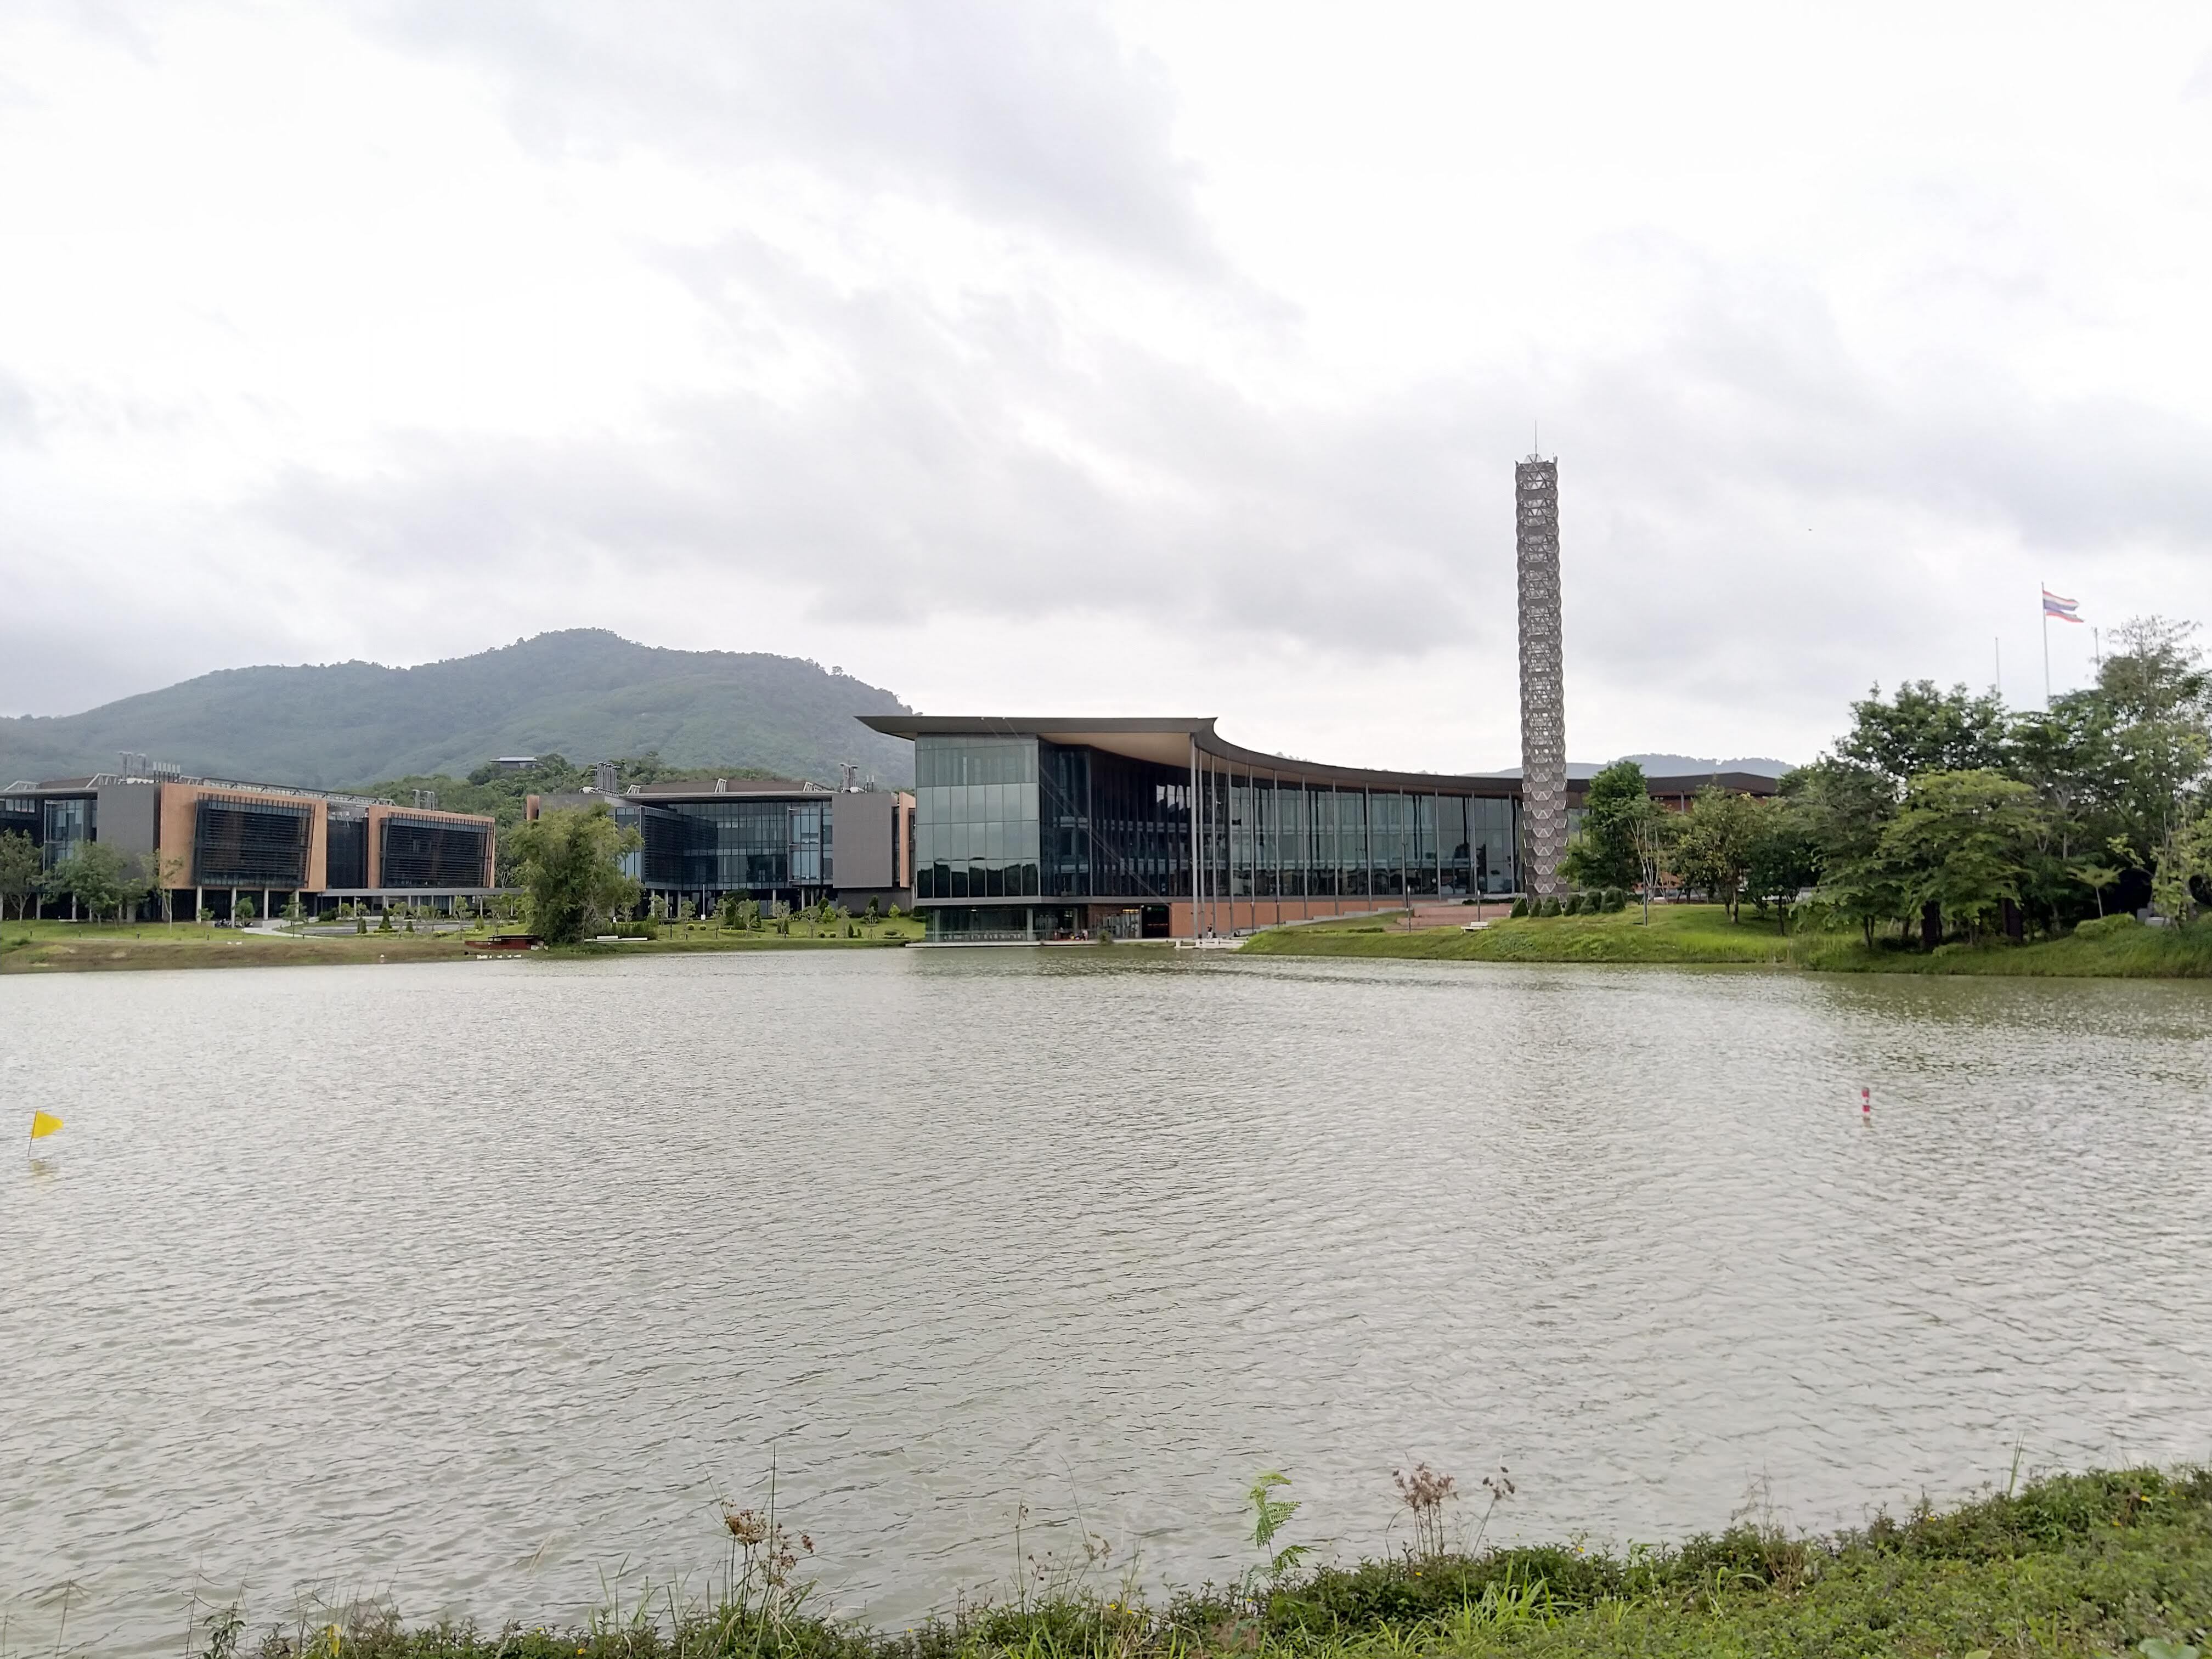
\includegraphics[width=0.8\textwidth]{images/vistec_v.jpg}
    \caption{อาคารหอสมุด สถาบันวิทยสิริเมธี}
\end{figure}

\textbf{สถาบันวิทยสิริเมธี (VISTEC)} เป็นบัณฑิตวิทยาลัย (graduate school) ซึ่งมุ่งเน้นความเป็นเลิศในการทำวิจัย ตั้งอยู่ในพื้นที่วังจันทร์วัลเลย์ (Wangchan Valley) และเขตนวัตกรรมระเบียงเศรษฐกิจพิเศษภาคตะวันออก (Eastern Economic Corridor of Innovation: EECi) เลขที่ 555 หมู่ 1 ตำบลป่ายุบใน อำเภอวังจันทร์ จังหวัดระยอง ก่อตั้งขึ้นเมื่อปี พ.ศ. 2558 โดยมูลนิธิพลังสร้างสรรค์นวัตกรรม ภายใต้การสนับสนุนเงินทุนจากบริษัทในกลุ่มของการปิโตรเลียมแห่งประเทศไทย (ปตท.)

VISTEC มุ่งเน้นการจัดการศึกษาด้านวิทยาศาสตร์ วิศวกรรม และเทคโนโลยี โดยมีศูนย์วิจัยวิทยาศาสตร์และเทคโนโลยีชั้นแนวหน้า (Frontier Research Center) ซึ่งเป็นศูนย์กลาง ในการเสริมสร้างความเข้มแข็งทางการวิจัย และให้การสนับสนุนด้านทุนการวิจัยแก่สถาบันฯ เป็นศูนย์รวมนักวิจัยที่มีความเชี่ยวชาญสูง ช่วยขับเคลื่อนการดำเนินงานด้านการศึกษา วิจัย การสร้างนวัตกรรม สร้างความร่วมมือทางด้านวิจัยกับสถาบันการศึกษา ภาคธุรกิจ ภาคอุตสาหกรรม
และหน่วยงานด้านการวิจัยวิทยาศาสตร์และเทคโนโลยี

\begin{figure}[H]
    \centering
    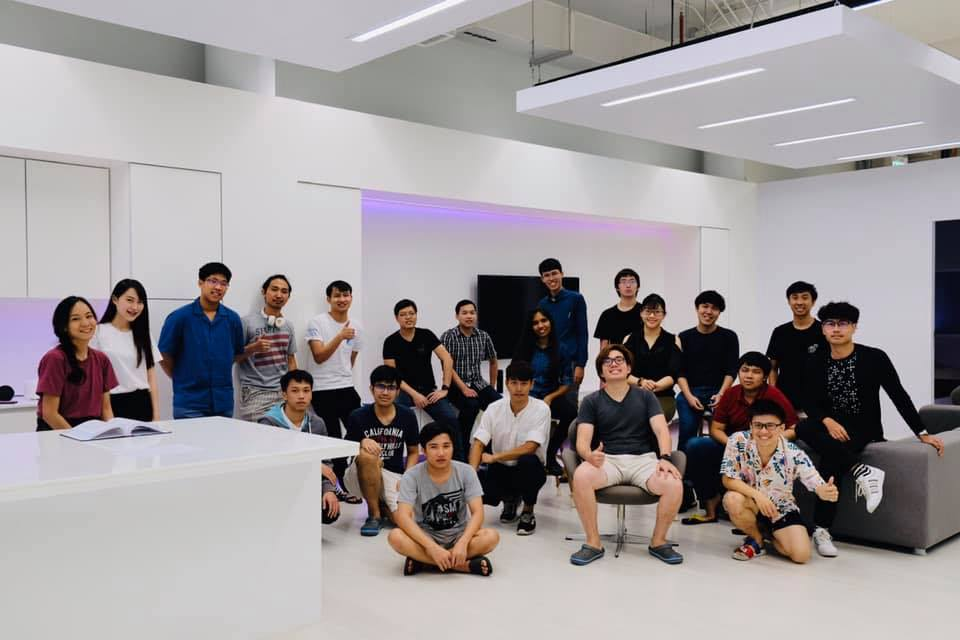
\includegraphics[width=0.8\textwidth]{images/brain_team_2019.jpg}
    \caption{ทีมวิจัย Interfaces, ห้องปฏิบัติการ BRAIN}
\end{figure}

\textbf{ห้องปฏิบัติการเบรน (Bio-inspired Robotics and Neural Engineering: BRAIN)}
ณ สำนักวิชาวิทยาศาสตร์และเทคโนโลยีสารสนเทศ สถาบันวิทยสิริเมธี มุ่งเน้นศึกษาการสร้างหุ่นยนต์ที่มีลักษณะร่วมกับกายวิภาค (anatomy) ของสิ่งมีชีวิต และใช้เทคโนโลยีจำพวก Machine Learning หรือ Deep Learning ในการจำแนก วิเคราะห์ และประมวลผลคลื่นสมองของมนุษย์ เพื่อสร้างส่วนติดต่อผู้ใช้ผ่านสมอง (Brain Controlled Interfaces: BCIs)

ลักษณะงานที่ได้รับผิดชอบจากห้องปฏิบัติการฯ เป็นงานของผู้ช่วยนักวิจัย (Research Assistant: RA) ซึ่งช่วยนิสิตระดับบัณฑิตศึกษาในการเตรียมการทดลอง ออกแบบ และพัฒนาเครื่องมือวัดผล ควบคุมการทดลอง และทดสอบสมมติฐานเพื่อตีพิมพ์องค์ความรู้ในวารสารวิชาการต่อไป

ที่ปรึกษาและผู้ควบคุมการฝึกงานในครั้งนี้ คืออ. ดร. ธีรวิทย์ วิไลประสิทธิ์พร หัวหน้าหน่วยวิจัย (Principal Investigator: PI) และมีระยะเวลาปฏิบัติงานประมาณ 2 เดือน กล่าวคือตั้งแต่วันที่ 4 มิถุนายน ถึง 31 กรกฎาคม 2562

\section{ประโยชน์ที่คาดว่าจะได้รับ}
เป็นการสร้างพื้นฐานในด้านงานวิจัย รวมถึงเตรียมพื้นฐานในการทำโครงงานวิศวกรรมคอมพิวเตอร์ โดยมีความมุ่งหวังจะต่อยอดงานดังกล่าวเป็นงานวิจัยตีพิมพ์ต่อไป

\chapter{ความรู้พื้นฐานและการทบทวนวรรณกรรม}
\section{ตัวชี้วัดทางชีวภาพ (Biomarkers)}
ตัวชี้วัดทางชีวภาพ (biomarkers) เป็นตัวบ่งชี้ต่อสภาวะต่างๆ ที่เกิดกับร่างกาย ซึ่งรวมถึงแต่ไม่จำกัดเพียงแต่สถานะการตื่น สภาพอารมณ์ หรือสัญญาณบ่งชี้ของโรค

\section{คลื่นสัญญาณชีวภาพ (Biosignals)}
คลื่นสัญญาณชีวภาพ (biosignals) เป็นคลื่นสัญญาณจากกระแสไฟฟ้าในร่างกาย ซึ่งสามารถตรวจวัดได้ด้วยวิธีการที่ต่างกันไป และผลจากการตรวจวัดคลื่นแต่ละส่วนจะบ่งบอกซึ่งข้อมูลที่แตกต่างกันออกไปเช่นกัน

\section{คลื่นไฟฟ้าสมอง (Electroencephalography)}
Electroencephalography หรือ EEG เป็นคลื่นที่เกิดจากการตรวจวัดกระแสไฟฟ้าของสมอง การตรวจวัดโดยมากไม่จำเป็นต้องทำการเจาะผิวหนัง (noninvasive) โดยใช้อิเล็กโทรดนำไฟฟ้าอ่านคลื่นสมองจากกระโหลก

การตรวจวัดและใช้ข้อมูลจากคลื่น EEG ส่วนมากมุ่งเน้นการใช้ศักย์ไฟฟ้าที่ขึ้นกับเหตุการณ์กระตุ้นของผู้ถูกวัด (Event Related Potential)  กล่าวคือมุ่งสังเกตจุดสูงสุดและต่ำสุดของศักย์ไฟฟ้าของคลื่นสมอง
และหาความสัมพันธ์ระหว่างเหตุการณ์กระตุ้นและการเพิ่มขึ้นหรือลดลงของศักย์ไฟฟ้า

\begin{figure}[h]
	\centering
	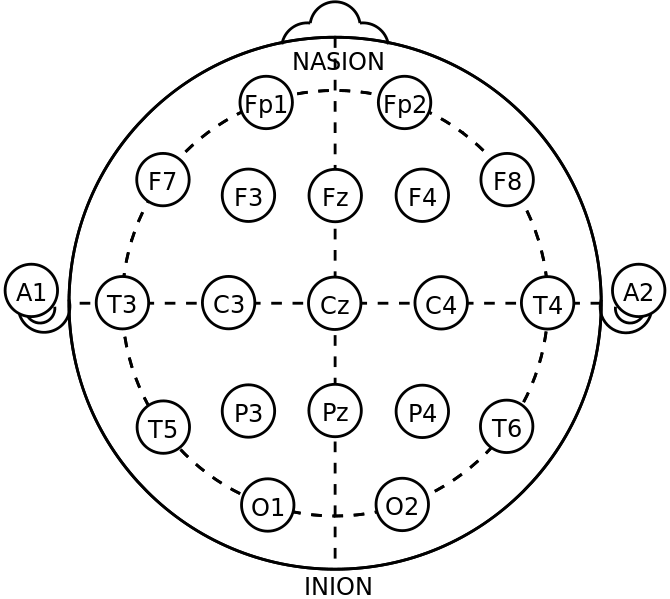
\includegraphics[width=0.5\textwidth]{images/1020.png}
	\caption{ภาพตำแหน่งของการติดขั้วนำไฟฟ้า (electrode) ตามระบบ International 10/20}
	\hspace{\linewidth}
	\textit{รูปภาพประกอบโดยผู้ใช้ Tomaton124 \href{https://commons.wikimedia.org/wiki/File:21_electrodes_of_International_10-20_system_for_EEG.svg}{บนโครงการวิกิมีเดีย คอมมอนส์}
		ชิ้นงานเป็นสาธารณะสมบัติ}
\end{figure}

อย่างไรก็ตาม การใช้คลื่นไฟฟ้านั้นยังสามารถใช้ประโยชน์จากคลื่นส่วนอื่น อันได้แก่คลื่นส่วน Motor Cortex ซึ่งถูกกระตุ้นด้วยการ "จินตนาการ"
การขยับร่างกาย และการใช้คลื่นส่วน Vision Cortex เพื่อกระตุ้นการมองเห็น เช่นการใช้สัญญาณ SSVEP จากสมองส่วนท้ายทอยซึ่งจะสั่นพ้อง
กับการกระพริบของแสงในความถี่ที่ตามองเห็น

\section{คลื่นไฟฟ้าจากการขยับลูกตา (Electrooculography)}
Electrooculography หรือ EOG เป็นคลื่นไฟฟ้าที่เกิดจากการขยับลูกตา โดยหากมองลูกตาเป็นวัตถุที่สามารถหมุนได้ด้วยองศาอิสระ (Degree of Freedom: DOF)
ทั้งหมด 2 องศาอิสระ สามารถจำความรู้นี้มาพิจารณาการใช้คลื่นจากกล้ามเนื้อการกอลกตาในการหาตำแหน่งการกลอกตาได้ \cite{bulling-eog}

\begin{figure}[h]
	\centering
	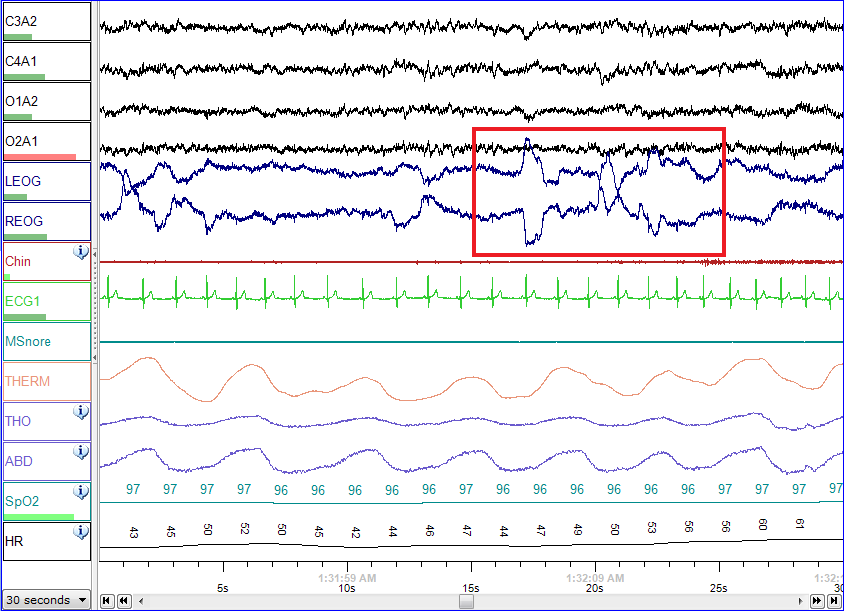
\includegraphics[width=0.7\textwidth]{images/rem_eog.png}
	\caption{ภาพคลื่น EOG ขณะอยู่ในสถานะการนอนหลับ}
	\hspace{\linewidth}
	\textit{รูปภาพประกอบโดยผู้ใช้ NascarEd \href{https://commons.wikimedia.org/wiki/file:sleep\_stage\_rem.png}{บนโครงการวิกิมีเดีย คอมมอนส์}
		สัญญาอนุญาต Creative Commons Attribution-Share Alike 3.0 Unported}
\end{figure}

การวัดคลื่น EOG สามารถทำได้ด้วยการติดอิเล็กโทรดจำนวน 2 คู่ เพื่อวัดการกลอกตาในแนวระนาบ (yaw) และการกลอกตาในแนวดิ่ง (pitch)
โดยค่าที่อ่านได้จากอิเล็กโทรดหนึ่งคู่จะเป็นการกลอกตาในทิศทางหนึ่ง กล่าวคือการวัด EOG มุ่งสนใจความต่างศักย์ไฟฟ้าของอิเล็กโทรดคู่นั้น
โดยการกลอกตาไปทางซ้าย (หรือกาารกลอกตาขึ้น) จะให้ทิศทางของตวามต่างศักย์ไฟฟ้าที่ต่างจากการกลอกตาไปทางขวา (หรือการกลอกตาลง)

\section{PERCLOS}
PERCLOS \cite{perclos} เป็นหนึ่งในวิธีการวัดความว่งง โดยใช้การวัดอัตราส่วนเวลาขณะตาปิดมากกว่าร้อยละ 70 หรือ 80 เทียบกับเวลาทั้งหมด เรียกมาตรวัดทั้งสองตัวว่า PERCLOS-70 และ PERCLOS-80 ตามลำดับ

\section{การติดตามดวงตา}

การติดตามดวงตา (eye tracking) \cite{eyetrack} จำเป็นต้องใช้เครื่องมือเฉพาะสำหรับการติดตาม เรียกอุปกรณ์ดังกล่าวว่าอุปกรณ์ติดตามดวงตา (eye tracker) ซึ่งมีโดยหลักสองประเภท ได้แก่อุปกรณ์แบบติดตั้งนิ่ง (fixed installation) และอุปกรณ์แบบสวมหัว (head-mounted)

การใช้อุปกรณ์ติดตามดวงตา จำเป็นจะต้องใช้ความระมัดระวังเป็นอย่างยิ่ง เนื่องจากสภาวะแสง สภาพการติดตั้ง และปัจจัยของผู้ทดลอง ส่งผลกระทบต่อการอ่านและประมวลผลได้โดยง่าย ยกตัวอย่างเช่น

\begin{itemize}
	\item ไม่ควรวางอุปกรณ์บนโต๊ะร่วมกับเมาส์และคีย์บอร์ด เนื่องจากการกดเมาส์และคีย์บอร์ดจะทำให้อุปกรณ์สั่น
	\item ผู้ทดลองไม่ควรใส่แว่นหรือคอนแทคเลนส์ เพราะจะทำให้การอ่านค่าผิดเพี้ยน
\end{itemize}
\section{การวัดคลื่นไฟฟ้าบนร่างกาย}

อุปกรณ์วัดคลื่นไฟฟ้าบนร่างกายโดยส่วนมากมักเป็นอุปกรณ์ทางการแพทย์ (medical equipments) ซึ่งต้องมีความแม่นยำและ
ความถูกต้องสูง เนื่องจากความถูกต้องในการอ่านค่าเพื่อวินิจฉัยโรคเป็นสิ่งสำคัญ จะผิดพลาดไม่ได้

อย่างไรก็ดี กระแสของ "นักสร้าง" (makers) ในกลุ่มนักพัฒนาและผู้สนใจในเทคโนโลยี ทำให้การเข้าถึงอุปกรณ์ดังกล่าวเป็นไปได้ง่ายขึ้น
เนื่องด้วยมีความพยายามในการสร้างฮาร์ดแวร์เปิดซอร์ส (open-source hardware) สำหรับวัดคลื่นดังกล่าว

\subsection{โอเพนบีซีไอ (OpenBCI)}

(Todo: OpenBCI image)
 
โอเพ่นบีซีไอ (OpenBCI) เป็นฮาร์ดแวร์แบบเปิดซอร์ส (open-source harware) สำหรับการวัดค่าทางชีวภาพ (biosensing)
อันได้แก่ค่าศักย์ไฟฟ้าในร่างกายมนุษย์ ตัวฮาร์ดแวร์เปิดแบบผังออกมาในลักษณะเดียวกับที่อาร์ดูโน่ (Arduino)
เปิดผังการออกแบบวงจรเป็นสาธารณะ

โอเพ่นบีซีไอสามารถใช้ในการวัดค่าความต่างศักย์ไฟฟ้าซึ่งเกิดจากทั้งสมอง (EEG) กล้ามเนื้อ (EMG) และหัวใจ (EKG)
โดยตัวบอร์ดเป็นวงจรตรรกะแบบ 32 บิทซึ่งใช้ชิป ADS1229 สำหรับการวัดค่าไฟฟ้าร่างกาย ผลิตโดยบริษัท Texas Instruments
และรองรับการวัดช่องสัญญาณได้สูงสุด 8 ช่องสัญญาณพร้อมกัน

\subsection{อิเล็กโทรด (Electrode)}

\begin{figure}[h]
    \centering
    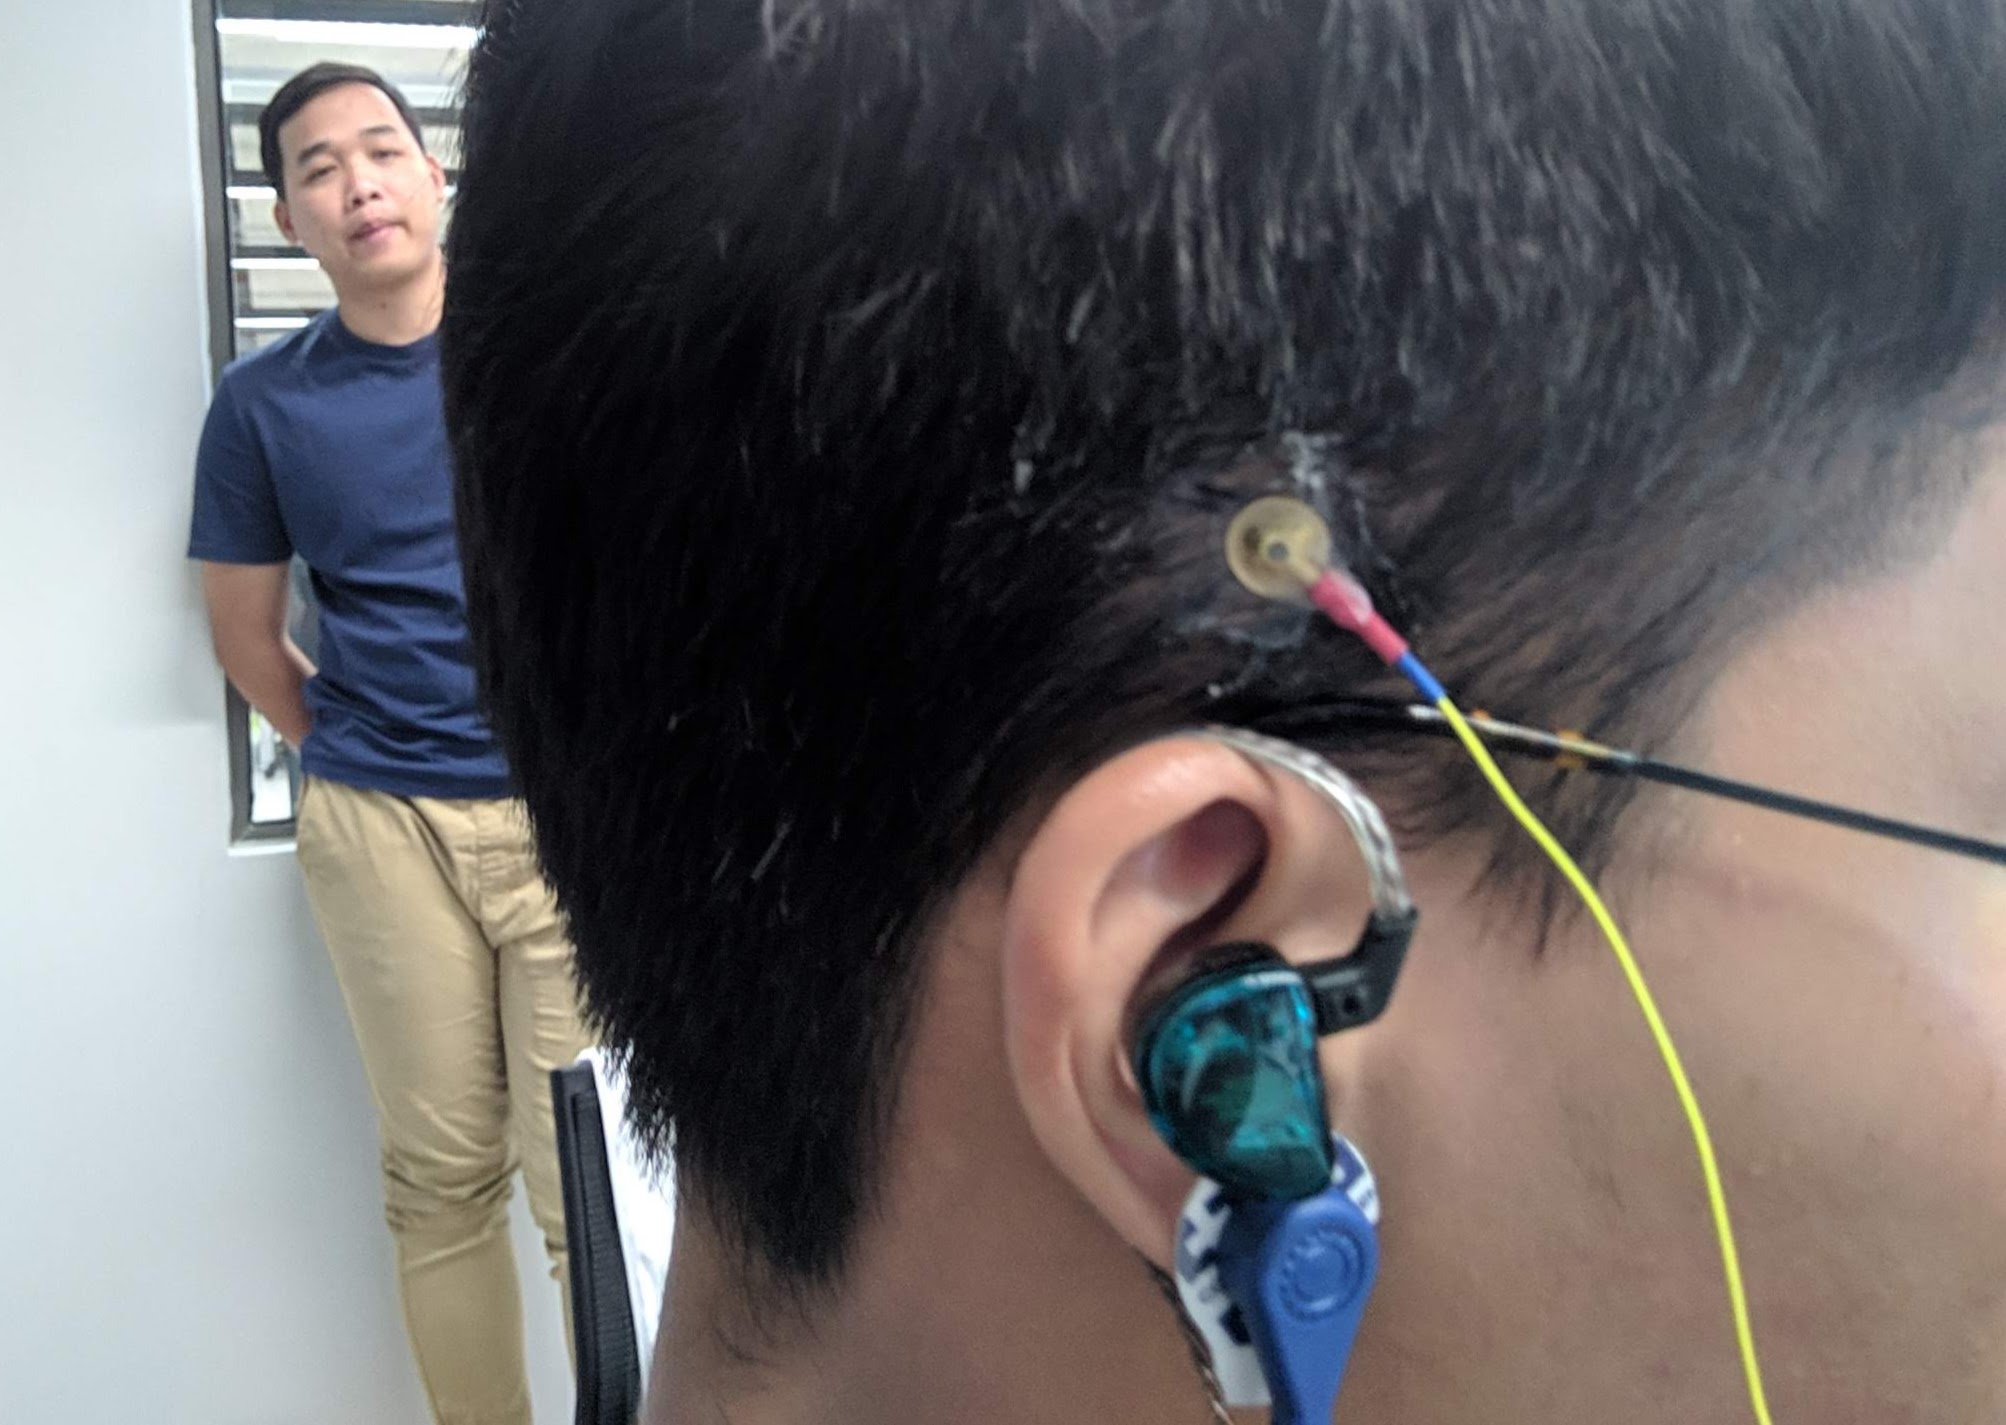
\includegraphics[width=0.5\textwidth]{images/IMG_20190610_155141.jpg}
    \caption{จากบนลงล่าง: อิเล็กโทรดแบบถ้วยทอง (Gold Cup) พร้อมสายสีเหลือง, หูฟัง, และอิเล็กโทรดแบบเจง (Gel) บริเวณติ่งหู}
\end{figure}

อิเล็กโทรดคือขั้วไฟฟ้าที่ทำการติดบนผิวหนังเพื่อวัดค่าศักย์ไฟฟ้าบริเวณจุดต่างๆ ที่สนใจ โดยมากมักใช้อิเล็กโทรดแบบ\textbf{ถ้วยทอง}
(Gold cup electrodes) และแบบ\textbf{เจล} (Get electrodes) ซึ่งสามารถเทียบกันได้ดังนี้

\begin{table}[h]
    \begin{tabularx}{\textwidth}{l|X|X}
                          & แบบถ้วยทอง                                           & แบบเจล                                                                           \\
                          \hline
    การทำความสะอาดผิวหนัง & \multicolumn{2}{l}{ต้องทำความสะอาดผิวหนังก่อน}                                                                                          \\
                          \hline
    การติดอิเล็กโทรด      & ต้องใช้ยานำไฟฟ้าผิวหนัง (skin conducting paste) เสมอ & อาจไม่ใช้ยานำไฟฟ้าผิวหนัง (skin conducting paste) แต่การใช้จะให้ผลลัพธ์ที่ดีกว่า \\
                          \hline
    ความง่ายในการติด      & ติดง่ายกว่าบริเวณที่มีผมหนา                          & ติดผิวหนังยากกว่าหากมีผมหนา                                                      \\
                          \hline
    ความเปรอะเปื้อน       & มาก เพราะยานำไฟฟ้าผิวหนังจะติดบริเวณผมและศีรษะ       & น้อย เจลสามารถลอกออกได้จากผิวหนังโดยไม่ทิ้งคราบ                                  \\
                          \hline
    ราคา                  & ถูกกว่า ใช้ซ้ำได้                                    & แพงกว่า ส่วนเจลใช้ได้ครั้งเดียว                                                 
    \end{tabularx}
\end{table}

\section{การเรียนรู้เชิงลึก (Deep Learning)}
การเรียนรู้เชิงลึก (Deep Learning) คือความพยายามในการจำลองเซลล์ประสามของมนุษย์ให้อยู่ในรูปโมเดลคณิตศาสตร์
ด้วยความเชื่อทางหลักประสาทวิทยา (neurosciences) ว่าความฉลาดของสมองมนุษย์เกิดขึ้นได้จากโครงข่ายประสาทจำนวนมาก
ที่เชื่อมเข้าถึงกัน

\subsection{เปอร์เซปตรอน (Perceptron)}
\begin{figure}[h]
    \centering
    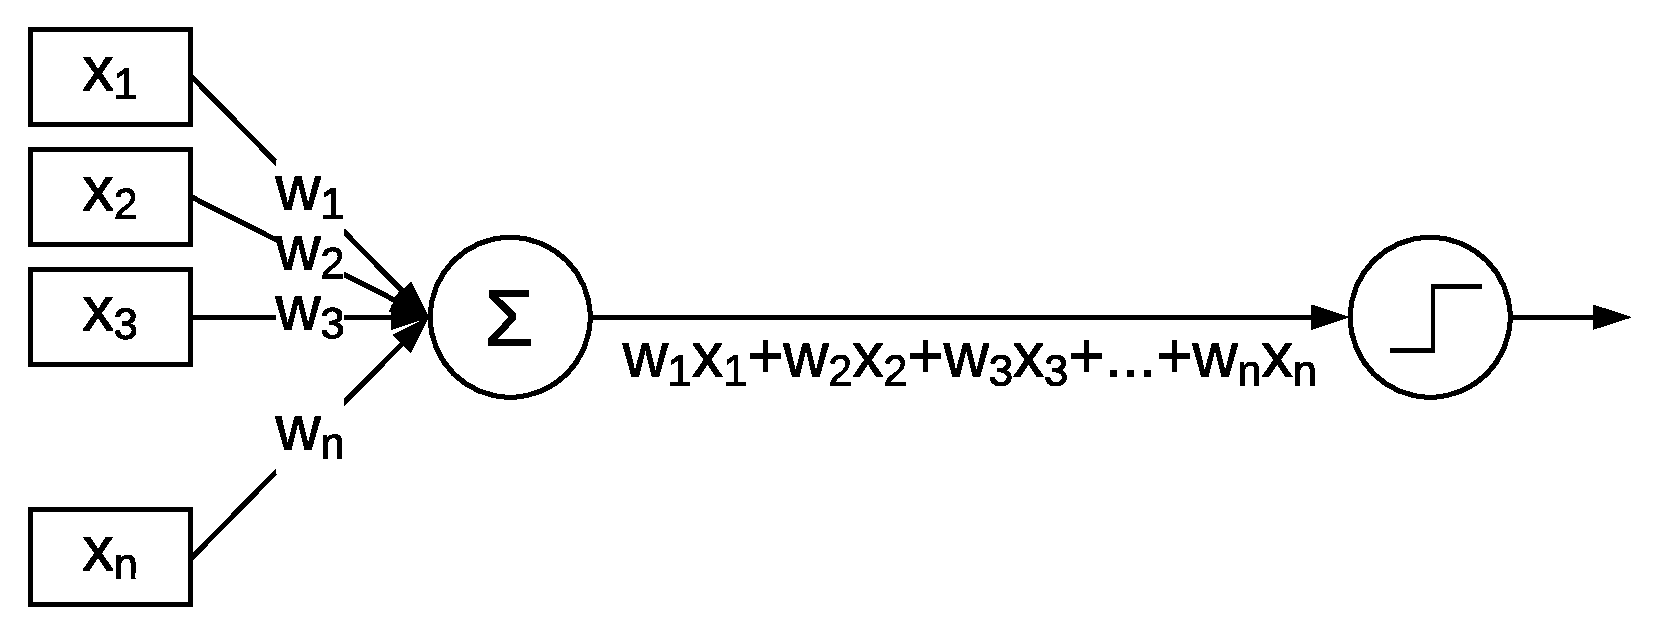
\includegraphics[width=0.7\textwidth]{images/perceptron.pdf}
    \caption{เปอร์เซปตรอน}
    \label{perceptron}
\end{figure}
เปอร์เซปตรอน (Perceptron) เป็นแบบจำลองทางคณิตศาสตร์ของเซลล์สมองหนึ่งเซลล์ โดยมีคุณสมบัติดังนี้

\begin{itemize}
    \item รับเข้าข้อมูลมาในเซลล์จากหลายแหล่ง และให้น้ำหนักกับข้อมูลนั้นต่างกันไป
    \item ส่งออกข้อมูลเพียงค่าเดียว
\end{itemize}

ดังนั้น แบบจำลองทางคณิตศาสตร์สามารถเขียนออกมาจากหลักการสองข้อดังกล่าวได้ด้วยสมการ

$$ y = f\left(W^TX+b\right) $$

เมื่อ $W$ และ $X$ เป็นเวกเตอร์ขนาด $1 \times n$ (โดย $n$ เป็นจำนวนข้อมูลรับเข้า), $b$ เป็นค่าสัมประสิทธิ์คงที่ (ไบแอส: bias)
และ $f$ เป็นฟังก์ชั่นกระตุ้น (activation function) ซึ่งอาจเขียนรูปร่างของเปอร์เซปตรอนให้มีลักษณะรูปคล้ายเซลล์สมองได้ในลักษณะรูปที่ \ref{perceptron}

ยกตัวอย่างการใช้เปอร์เซปตรอนในการแก้ปัญหาอย่างง่ายได้ในที่นี้

\subsubsection{การคาดเดาราคาอสังหาริมทรัพย์}
หากสำรวจราคาอสังหาริมทรัพย์แล้วพบว่า
\begin{itemize}
    \item ราคาอสังหาริมทรัพย์จะเพิ่มขึ้นตามที่ดิน โดยเพิ่มขึ้นทุก 10,000 บาทต่อตารางวา
    \item ราคาอสังหาริมทรัพย์จะเพิ่มขึ้นตามจำนวนห้องนอน โดยเพิ่มขึ้นทุก 200,000 บาทต่อห้องนอน
    \item ราคาอสังหาริมทรัพย์จะลดลงตามจำนวนอายุปี โดยลดลงทุก 7,000 บาทต่ออายุของอสังหาริมทัพย์
\end{itemize}
\noindent
จะสามารถเขียนเปอร์เซปตรอนเพื่อคาดเดาราคาอสังหาริมทรัพย์ได้โดย
$$ y = f\left(W^TX+b\right) $$
เมื่อ $W$ ซึ่งเป็นค่าสัมประสิทธิ์แสดงถึงความสัมพันธ์ข้อมูลรับเข้า ซึ่งเขียนได้จากความสัมพันธ์ดังแสดงด้านล่าง
$$
    W^T = \begin{bmatrix}
        10000 & 200000 & -7000
    \end{bmatrix}
$$
$b$ เป็นไบแอส, จะสมมติให้ $b = 0$ (กล่าวโดยละเอียด ในที่นี้ $b$ คือราคาตั้งต้นของบ้าน 0 ห้องนอน พื้นที่ 0 ตารางวา อายุ 0 ปี) และ $f(x) = x$ กล่าวคือเป็นฟังก์ชั่นเชิงเส้น

หากต้องการคาดเดาราคาบ้านที่มี 3 ห้องนอน เนื้อที่ 100 ตารางวา และมีอายุ 7 ปี จะสามารถเขียนเวกเตอร์ $P$ ได้เป็น

$$
    X = \begin{bmatrix}
        3 \\
        100 \\
        7
    \end{bmatrix}
$$
และผลการทำนายราคาบ้านคำนวนได้จาก
$$
    \begin{aligned}
        y &= f\left(W^TX+b\right)\\
        &= f\left(\begin{bmatrix}
            10000 & 200000 & -7000
        \end{bmatrix} \times \begin{bmatrix}
            3 \\
            100 \\
            7
        \end{bmatrix}\right)\\
        &= f(30000 + 20000000 + (-49000)) = f(19981000)\\
        &= 19981000
    \end{aligned}
$$

\subsubsection{การสร้างประตูสัญญาณตรรกะด้วยเปอร์เซปตรอน}
เราสามารถสร้างประตูสัญญาณตรรกะ (logic gates) บางชนิดได้ด้วยเปอร์เซปตรอน เช่นการสร้าง AND และ OR gate

ยกตัวอย่างโครงสร้างของ AND gate ซึ่งสามารถสร้างได้ด้วยการกำหนดให้
\begin{itemize}
    \item $X$ เป็นเมทริกซ์ขนาด $1 \times 2$ กล่าวคือเมื่อรับค่า $x_1, x_2$ เป็นค่า 0 หรือ 1 แทนสัญญาณจริงหรือเท็จแล้ว
        $$X = \begin{bmatrix}
            a_1 \\
            a_2
        \end{bmatrix}$$
    \item กำหนดค่าของเมทริกซ์ $W$ เป็น
        $$W^T = \begin{bmatrix}
            1 && 1
        \end{bmatrix}$$
    \item กำหนดค่าของไบแอส $b = -2$
    \item กำหนดฟังก์ชั่น $f(x)$ เป็น step function กล่าวคือ
    $$
        f(x) = \begin{cases}
            1; & x \geq 0\\
            0; & \textrm{ในกรณีอื่น}
        \end{cases}
    $$
\end{itemize}
และการสร้าง OR gate สามารถทำได้ในลักษณะเดียวกันโดยเปลี่ยน $b$ เป็น $b = -1$

\subsection{เปอร์เซปตรอนแบบหลายชั้น (Multi Layer Perceptron)}

เราอาจสังเกตว่าเปอร์เซพตรอนหนึ่งตัวนั้นทำหน้าที่ได้เพียนแยก (classify) หรือถดถอย (regress) ปัญหาที่เป็นปัญหาเชิงเส้น (linear problems) ได้เท่านั้น อย่างไนก็ตามหากเรากำหนดให้ฟังก์ชั่น $f$ เป็นฟังก์ชั่นที่ไม่ใช่ฟังก์ชั่นเส้นตรงแล้ว เราอาจสร้าง\textbf{เปอร์เซปตรอนแบบหลายชั้น} (Multi Layer Perceptron) ขึ้นมาได้โดยมีลักษณะดังรูปที่ \ref{mlp}

\begin{figure}
    \centering
    \def\layersep{2.5cm}
    \begin{tikzpicture}[->,draw=black!70, node distance=\layersep]
        \tikzstyle{every pin edge}=[<-,shorten <=1pt]
        \tikzstyle{neuron}=[circle,draw=black!100,minimum size=17pt, outer sep=3pt]
        \tikzstyle{annot}=[text width=5em, text centered]
    
        \foreach \name / \y in {1,...,4}
            \node[neuron, pin=left:ข้อมูลรับเข้า \y] (I-\name) at (0,-\y) {};
    
        % Draw the hidden layer nodes
        \foreach \name / \y in {1,...,5}
            \path[yshift=0.5cm]
                node[neuron] (HA-\name) at (\layersep,-\y cm) {};
    
        \foreach \name / \y in {1,...,5}
            \path[yshift=0.5cm]
                node[neuron] (HB-\name) at (2*\layersep,-\y cm) {};

        \foreach \name / \y in {1,...,3}
            \path[yshift=-0.5cm]
                node[neuron] (O-\name) at (3*\layersep,-\y cm) {};
    
        \foreach \source in {1,...,4}
            \foreach \dest in {1,...,5}
                \path (I-\source) edge (HA-\dest);
    
        \foreach \source in {1,...,5}
            \foreach \dest in {1,...,5}
                \path (HA-\source) edge (HB-\dest);

        \foreach \source in {1,...,5}
            \foreach \dest in {1,...,3}
                \path (HB-\source) edge (O-\dest);

        \node[annot,above of=I-1, node distance=1cm] (hla) {ชั้นรับเข้า (ชั้นที่ 0)};
        \node[annot,above of=HA-1, node distance=1cm] (hla) {ชั้นซ่อน 1};
        \node[annot,above of=HB-1, node distance=1cm] (hla) {ชั้นซ่อน 2};
        \node[annot,above of=O-1, node distance=1cm] (hlb) {ชั้นส่งออก (ชั้นที่ 3)};

    \end{tikzpicture}
    \caption{เปอร์เซปตรอนแบบหลายชั้น}
    \label{mlp}
\end{figure}

เราอาจเขียนแทนน้ำหนักของโครงข่ายจากเปอร์เซปตรอนชั้นที่ $i$ ไปยังชั้นที่ $j$ ($j=i+1$) ได้เป็น
\begin{equation*}
    \boldsymbol{W}_{ij} = 
    \begin{bmatrix}
        w_{11} & w_{21} & \dots & w_{n_{i}1}\\
        w_{12} & w_{22} & \dots & w_{n_{i}2}\\
        \vdots & \vdots & \ddots & \vdots\\
        w_{1n_j} & w_{2n_j} & \dots & w_{n_jn_i}
    \end{bmatrix}
\end{equation*}
เมื่อจำนวนเปอร์เซปตรอนในชั้นที่ $k$ เขียนแทนด้วย $n_k$

ยกตัวอย่างเช่น เราจะสามารถสร้างประตูสัญญาณ XOR (XOR gate) ได้จากเปอร์เซปตรอนแบบหลายชั้นดังแสดงในรูปที่ \ref{xor-mlp} โดยเลขในแต่ละเปอร์เซปตรอนแทนค่าไบแอส ($b$) และเลขบนเส้นเชื่อมแทนค่าน้ำหนัก ($w$) และกำหนดให้ฟังก์ชั่นกระตุ้น $f$ เป็นฟังก์ชั่นขั้นบันได (step function) กล่าวคือ
\begin{equation*}
    f(x) =
    \begin{cases}
        1; & x \geq 0\\
        0; & \textrm{ในกรณีอื่น}
    \end{cases}
\end{equation*}
เปอร์เซปตรอนดังกล่าว เมื่อรับค่า $A$ และ $B$ เป็น 0 หรือ 1 จะส่งออกค่า $A \oplus B$

\begin{figure}
    \def\layersep{2.5cm}
    \centering
    \begin{tikzpicture}[<-, draw=black!70, node distance=\layersep]
        \tikzstyle{edge}=[->,fill=white]
        \tikzstyle{neuron}=[circle,draw=black!100,minimum size=25pt, outer sep=3pt]
        \tikzstyle{annot}=[text width=5em, text centered]
    
        \node[neuron, pin=left:$A$] (I-1) at (0,0 cm) {$A$};
        \node[neuron, pin=left:$B$] (I-2) at (0,-2 cm) {$B$};
    
        \node[neuron] (HA-1) at (\layersep,-0 cm) {$-2$};
        \node[neuron] (HA-2) at (\layersep,-2 cm) {$-2$};

        \node[neuron] (O) at (2*\layersep,-1 cm) {$-1$};

        \path[edge]
            (I-1) edge node {$-1$} (HA-1)
            (I-1) edge node[very near end] {$1$} (HA-2)
            (I-2) edge node[very near end] {$1$} (HA-1)
            (I-2) edge node {$-1$} (HA-2)
            (HA-1) edge node {$1$} (O)
            (HA-2) edge node {$1$} (O)
        ;
    \end{tikzpicture}
    \caption{เปอร์เซปตรอนแบบหลายชั้นซึ่งทำหน้าที่เป็นประตูสัญญาณ XOR}
    \label{xor-mlp}
\end{figure}

\chapter{ระเบียบวิธีดำเนินงาน}
\section{การออกแบบการทดลอง}

\subsection{การทดลองเบื้องต้น}

\chapter{ผลลัพธ์และการวิเคราะห์ผล}

\chapter{บทสรุป}

\begin{appendices}
\chapter{บันทึกประจำวัน}
\section*{4/6/2562}

เนื่องจากเข้าทำงานเป็นวันแรก จึงต้องจัดสถานที่ทำงาน และทำงานต่อจากที่ได้รับมอบหมายก่อนการฝึกงาน

งานที่ได้รับมอบหมายโดยคร่าวคือการวิเคราะห์สภาวะความง่วงในคน โดยศึกษาจากกลุ่มเป้าหมายของพนักงานบริษัท
ซึ่งอาจารย์ที่ปรึกษาให้สิทธิ์ในการกำหนดแนวทางการวิเคราะห์ได้โดยอิสระ อย่างไรก็ตามงานของการวิเคราะห์ความง่วง
โดยตั้งต้นนั้นมักใช้การวิเคราะห์ภาพจากดวงตา (gaze monitoring) ซึ่งใช้วันนี้ในการหางานวิจัยตั้งต้น

นอกจากนี้ยังศึกษาแนวทาง ข้อกำหนด และมาตรฐานจริยธรรมในการทดลองภายในมนุษย์ (human subject research)

\section*{5/6/2562}

ศึกษาแนวทางในการทำ eye gazing ตามหนังสือที่ได้รับมอบหมาย และนำเสนองานวิจัยต่อจากที่เลือกจากเมื่อวาน

ปรับแก้แนวทางในการวิจัย และได้รับมอบหมายให้ออกแบบวิธีการทดลองโดยคร่าว
หารือกับทีมโปรแกรมเมอร์ว่าด้วยซอฟต์แวร์สำหรับการทดลอง

\section*{6/6/2562}

ศึกษาอุปกรณ์สำหรับติดตามดวงตา (Gazepoint) ก่อนจะพบว่าอุปกรณ์มีข้อจำกัดในการทำงานบางส่วน ทำให้ไม่สามารถดึง
ภาพดวงตาออกมาใช้ในโปรแกรมภายนอกได้ และติดต่อกับผู้ผลิตอุปกรณ์เพื่อหารือความเป็นไปได้ในการดึงภาพดวงตา

ศึกษาการใช้ Pytorch ในการทำการเรียนรู้เชิงลึก (deep learning) แทนที่ Keras

\section*{7/6/2562}

เปลี่ยนแนวทางการทำวิจัยด้วยข้อจำกัดของอุปกรณ์ มาเป็นการทำวิจัยบนกล้ามเนื้อตา (EOG) ค้นคว้าและทบทวนวรรรณกรรม
ที่เกี่ยวข้องกับงาน

ทำแบบทดสอบสำหรับบทเรียนจริยธรรมการวิจัยในมนุษย์จนอยู่ในเกณฑ์ได้รับประกาศนียบัตรผ่านการอบรม

\section*{10/6/2562}

นักเรียนจากโครงการพัฒนาอัจฉริยภาพทางวิทยาศาสตร์เข้ามาร่วมในทีม โดยการทดลองในส่วนของ Drowsiness research
ถูกแบ่งออกเป็นสองงานที่ต้องทดลองร่วมกัน จึงต้องตกลงแนวทางการทดลองให้ชัดเจน

ทดลองให้นักเรียนดังกล่าวศึกษาการวัดคลื่นสมองโดยอุปกรณ์ OpenBCI, ให้คำแนะนำถึงการเตรียมผิวหนัง (skin preparation)
ก่อนการติดอิเล็กโทรด, การเลือกใช้ชนิดอิเล็กโทรดและข้อดี-ข้อเสียของอิเล็กโทรดแต่ละชนิด

\section*{11/6/2562}

ทำงานที่ได้รับมอบหมายต่อจากเมื่อวาน

\section*{12/6/2562}

นัดประชุมงานกับอาจารย์ที่ปรึกษาโครงการ สรุปแนวทางการทดลอง และตัดสินใจเพิ่มการวัด PVT (Psychomotor vigilance task)
เพิ่มเติมในการทดลอง

เขียนโปรแกรมสำหรับทดสอบ PVT โดยใช้การสื่อสารบนอุปกรณ์หลายเครื่องเพื่อลดความจำเป็นในการซื้อปุ่ม (physical button)
ด้วยเหตุผลทางงบประมาณ

ช่วงเย็นรับประทานอาหารเย็นร่วมกับอาจารย์ธงชัย ชิวปรีชา

\section*{13/6/2562}

ได้รับมอบหมายให้ทดลองจับภาพตาเพื่อหา PERCLOS ด้วยกล้องเว็บแคมแบบที่มีหลอดอินฟราเรด ในเบื้องต้นสามารถครอปตัดเฉพาะส่วน
ที่เป็นลูกตาออกจากภาพใบหน้าแบบเต็มหน้าได้ อย่างไรก็ตาม ไม่ประสบความสำเร็จในการคำนวนร้อยละพื้นที่ของตาดำที่ไม่ถูกหนังตาบดบัง

\begin{figure}[H]
    \centering
    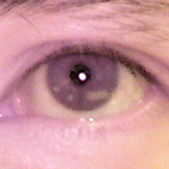
\includegraphics[width=0.4\textwidth]{images/268.png}
    \caption{ภาพถ่ายตาจากล้อง IR}
\end{figure}

\section*{14/6/2562}

ศึกษาและทบทวนวรรณกรรมว่าด้วยการประมวลผลภาพลูกตา และนำมาประยุกต์เขียนบนไลบรารี่ OpenCV จนสามารถสกัดตำแหน่งงของตาออกมา
จากภาพถ่ายของใบหน้าผู้ใช้ได้

ตัดสินใจเปลี่ยนจากเว็บแคมพร้อมหลอด IR เป็นกล้องธรรมดา

\begin{figure}[H]
    \centering
    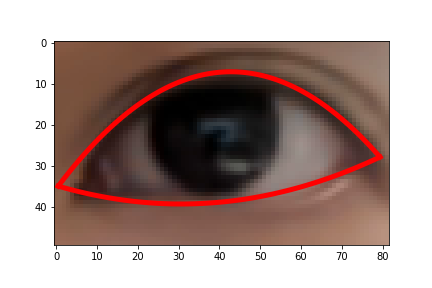
\includegraphics[width=0.4\textwidth]{images/111.png}
    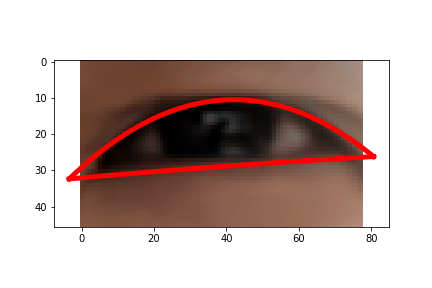
\includegraphics[width=0.4\textwidth]{images/171.png}
    \caption{ภาพถ่ายตาจากล้องที่ประมวลผลภาพเพื่อหาตำแหน่งของดวงตา ทั้งกรณีที่เปิดและปิดตา โดยประมวลผลภาพออกมาเป็นที่เรียบร้อย}
\end{figure}

\section*{17/6/2562}

ได้รับมอบหมายกระทันหันให้ร่วมเขียนเปเปอร์กับทีม SSVEP จีงเปลี่ยนสโคปงานเป็นการเขียนเปเปอร์ให้สามารถส่งตีพิมพ์ได้เร็วที่สุด

ศึกษาการใช้งานเครื่องมือทางสถิติ และทบทวนวรรณกรรมเท่าที่จำเป็น

\section*{18/6/2562}

เขียน ทบทวน และตรวจทานงานวิจัย

\section*{19/6/2562}

เขียน ทบทวน และตรวจทานงานวิจัยต่อ

\section*{20/6/2562}

เขียน ทบทวน และตรวจทานงานวิจัยต่อ

\section*{21/6/2562}

เขียน ทบทวน และตรวจทานงานวิจัยต่อ

\section*{24/6/2562}

เขียน ทบทวน และตรวจทานงานวิจัยต่อ

\section*{25/6/2562}

เขียน ทบทวน และตรวจทานงานวิจัยต่อ

\chapter{ภาพถ่ายสถานที่ปฏิบัติงาน}

\section*{ภาพการฝึกงานวันที่ 4/6/2562}
\begin{figure}[H]
    \centering
    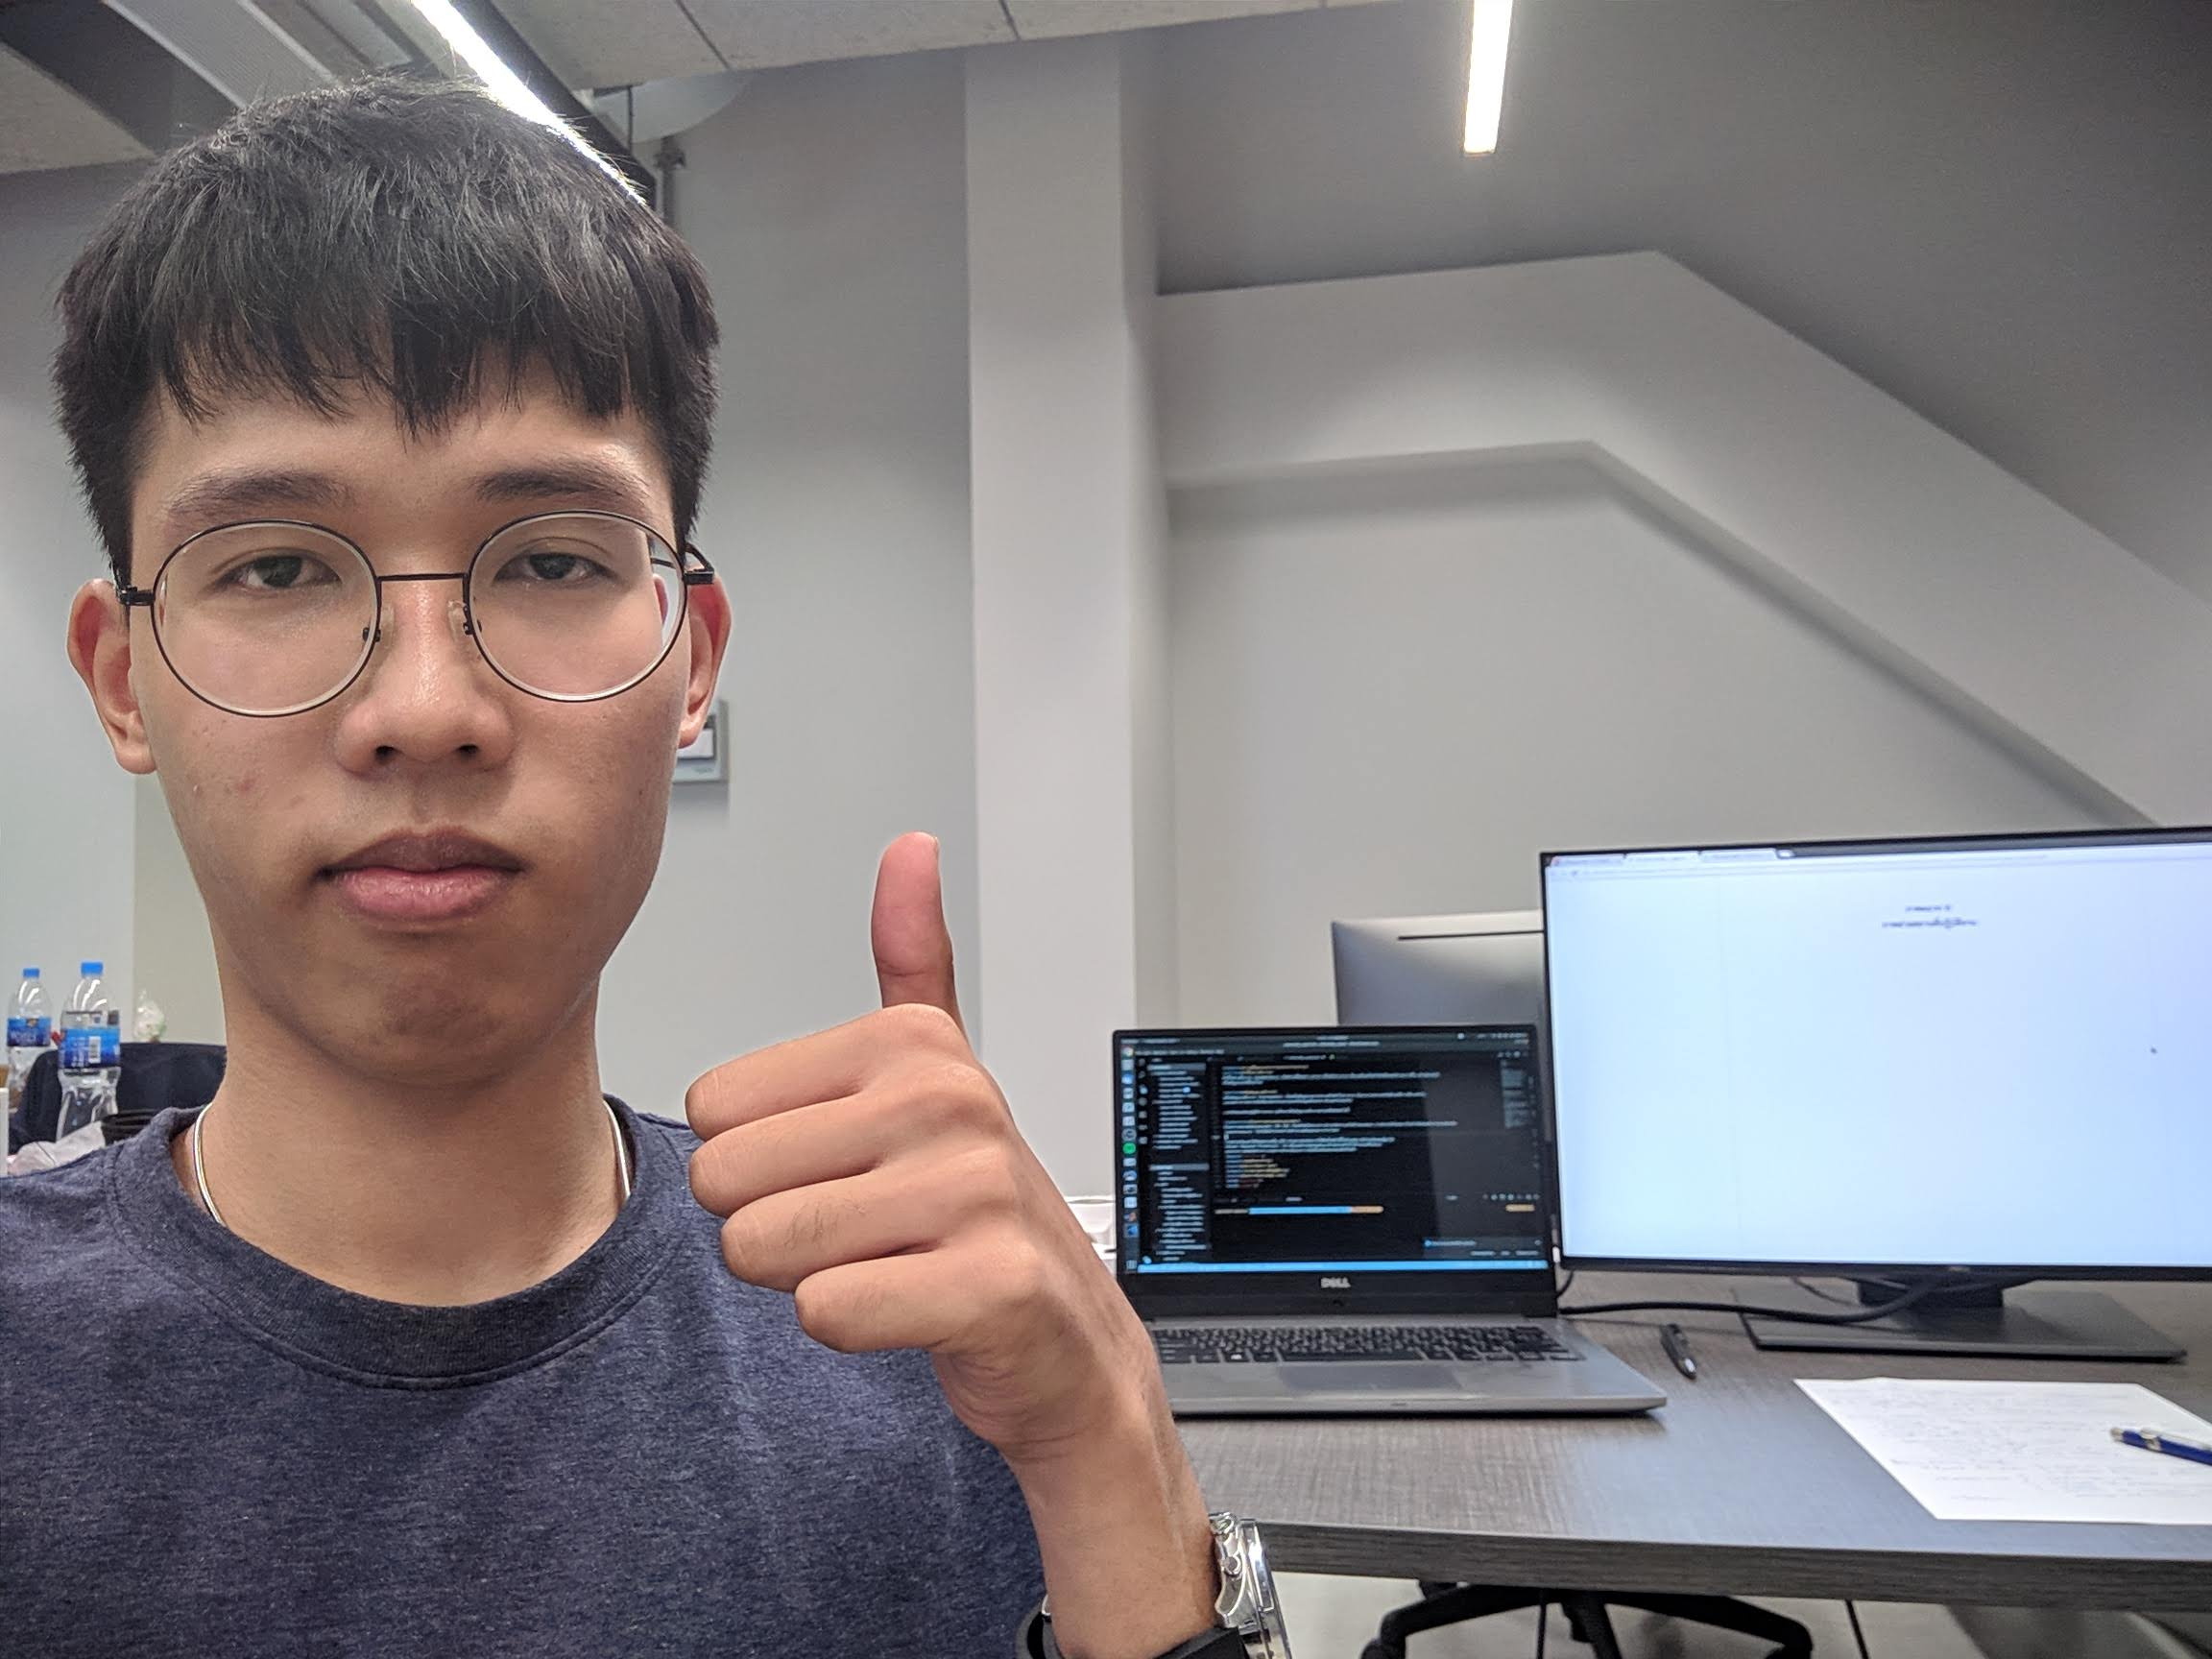
\includegraphics[width=0.55\textwidth]{/home/srakrn/Works/senior/internship/internship_report/diary/images/IMG_20190604_152401.jpg}
    \caption{สถานที่ทำงานหลังจากจัดที่ทำงานแล้ว}
\end{figure}

\section*{ภาพการฝึกงานวันที่ 5/6/2562}
\begin{figure}[H]
    \centering
    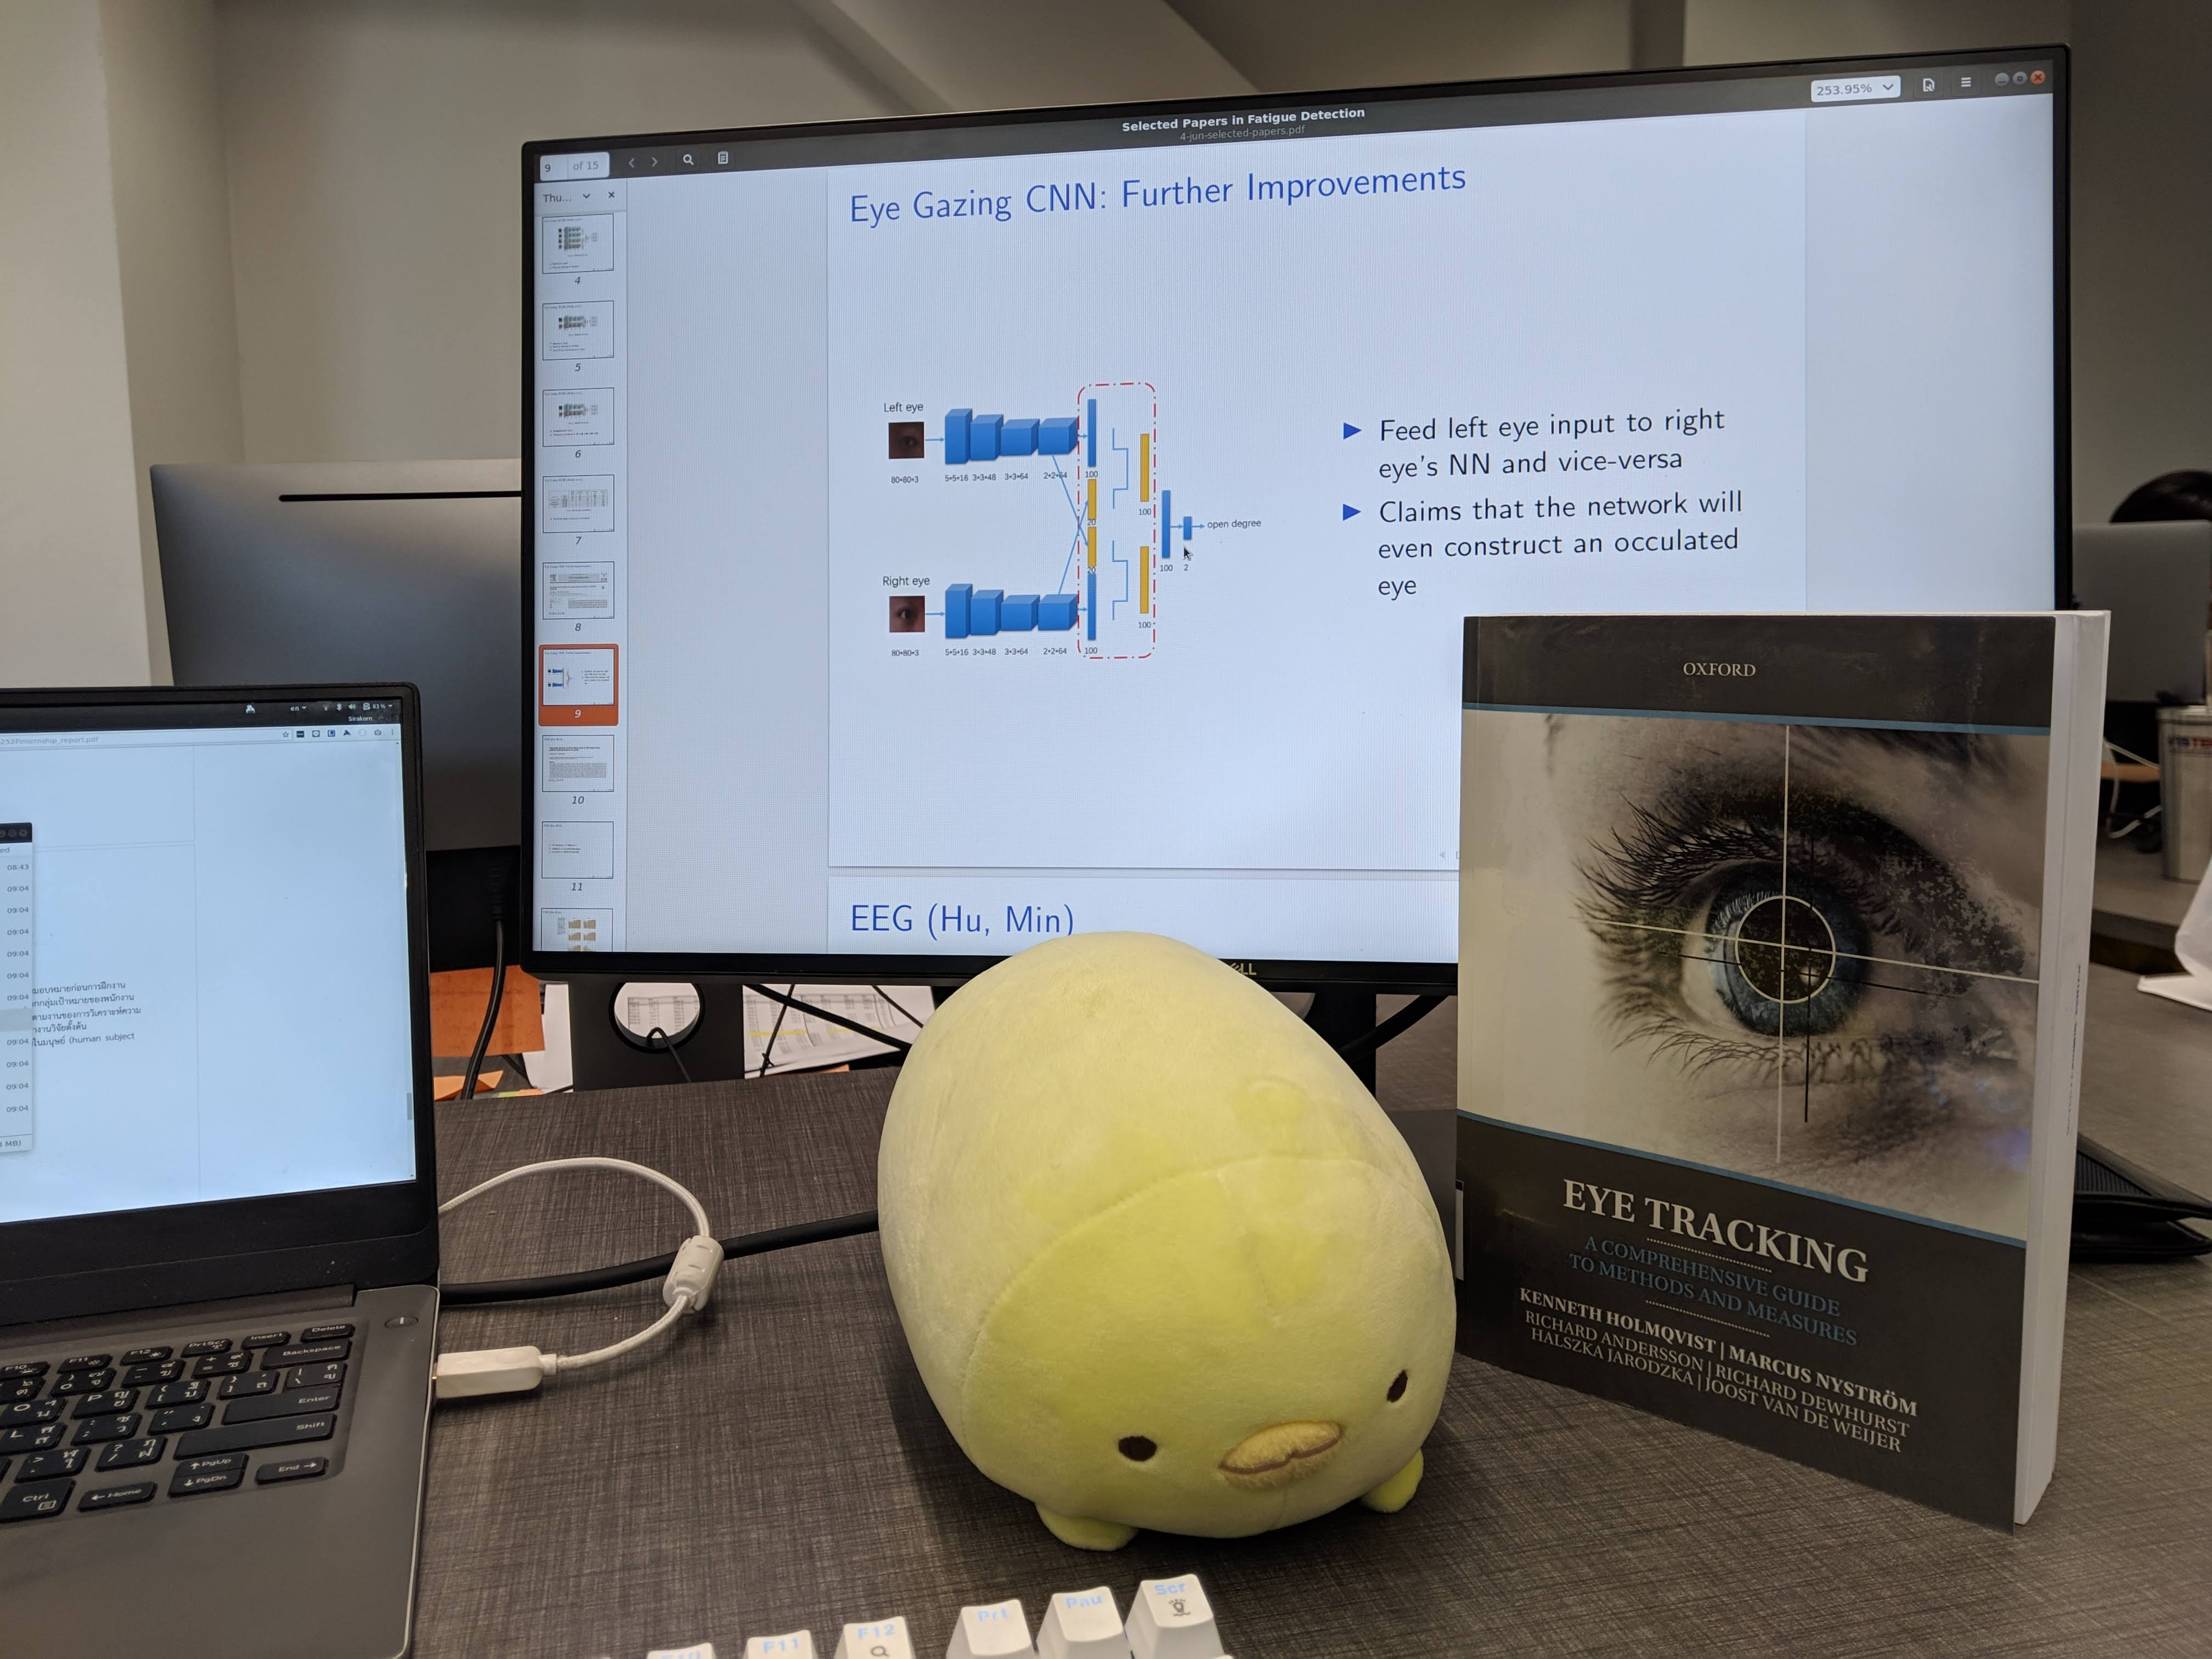
\includegraphics[width=0.55\textwidth]{/home/srakrn/Works/senior/internship/internship_report/diary/images/IMG_20190605_112217.jpg}
    \caption{หนังสือที่ได้รับมอบหมายให้อ่านและศึกษา ถ่ายคู่กับสไลด์สรุปงานวิจัย}
\end{figure}

\section*{ภาพการฝึกงานวันที่ 6/6/2562}
\begin{figure}[H]
    \centering
    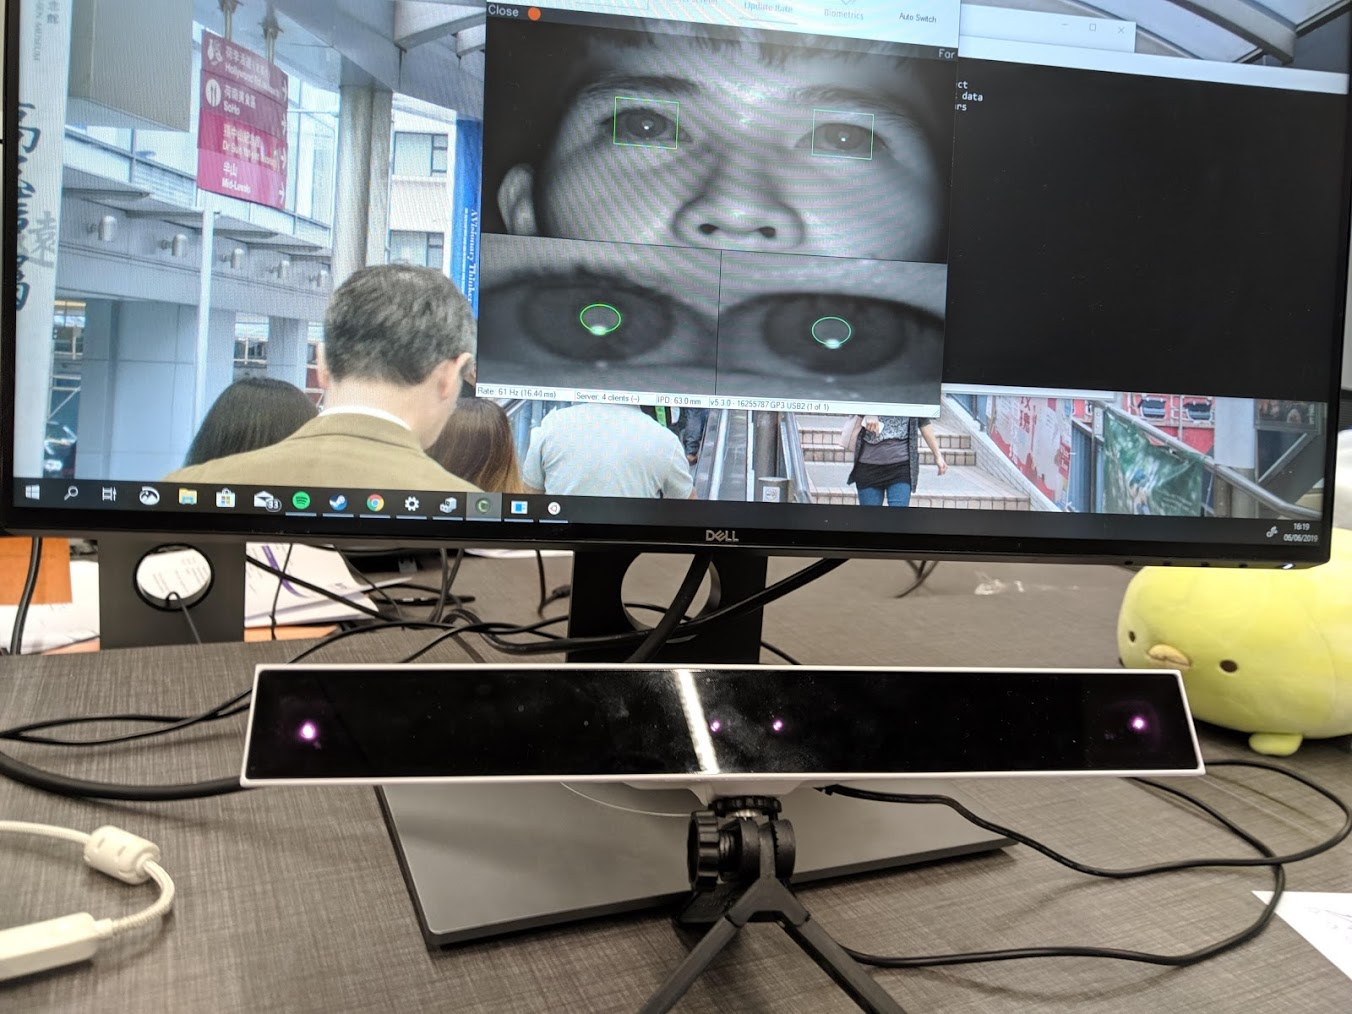
\includegraphics[width=0.55\textwidth]{/home/srakrn/Works/senior/internship/internship_report/diary/images/IMG_20190606_161925.jpg}
    \caption{อุปกรณ์สำหรับติดตามดวงตา Gazepoint ขณะกำลังจับม่านตา}
\end{figure}

\section*{ภาพการฝึกงานวันที่ 10/6/2562}
\begin{figure}[H]
    \centering
    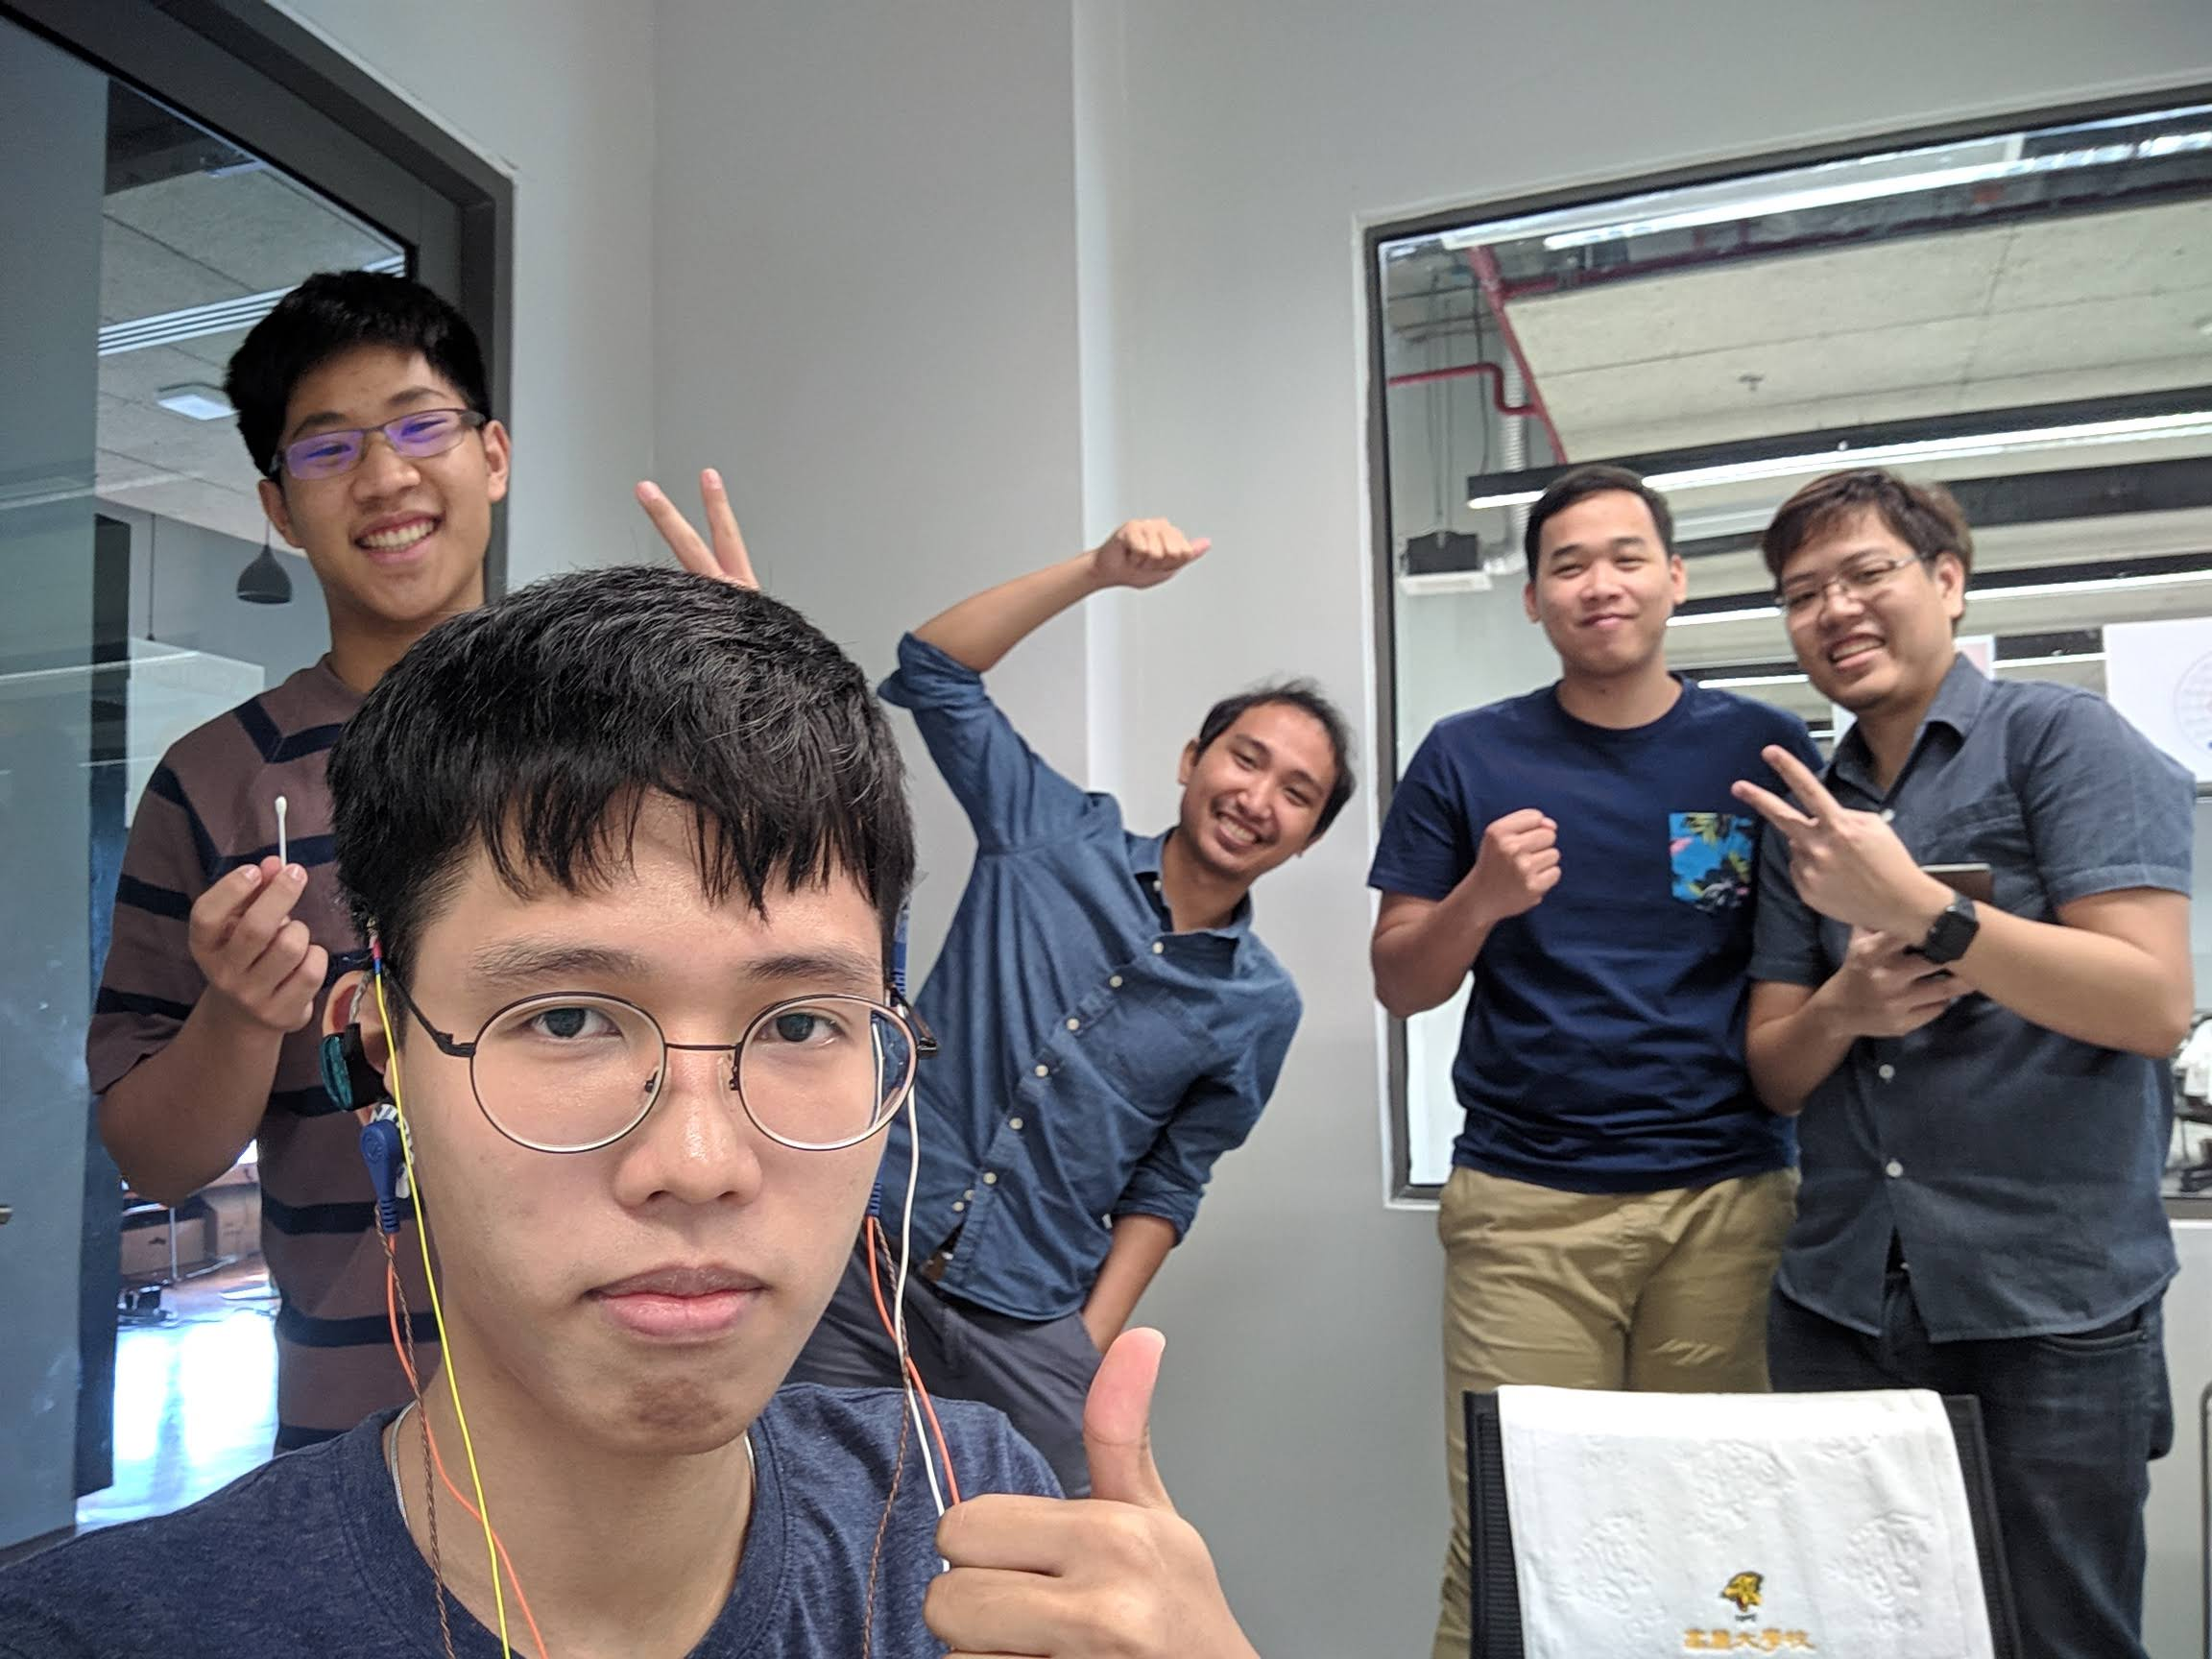
\includegraphics[width=0.55\textwidth]{/home/srakrn/Works/senior/internship/internship_report/diary/images/IMG_20190610_155035.jpg}
    \caption{สมาชิกทีม Drowsiness Research และสมาชิกทีม BRAIN ขณะทดสอบสมมติฐาน}
\end{figure}

\section*{ภาพการฝึกงานวันที่ 24/6/2562}
\begin{figure}[H]
    \centering
    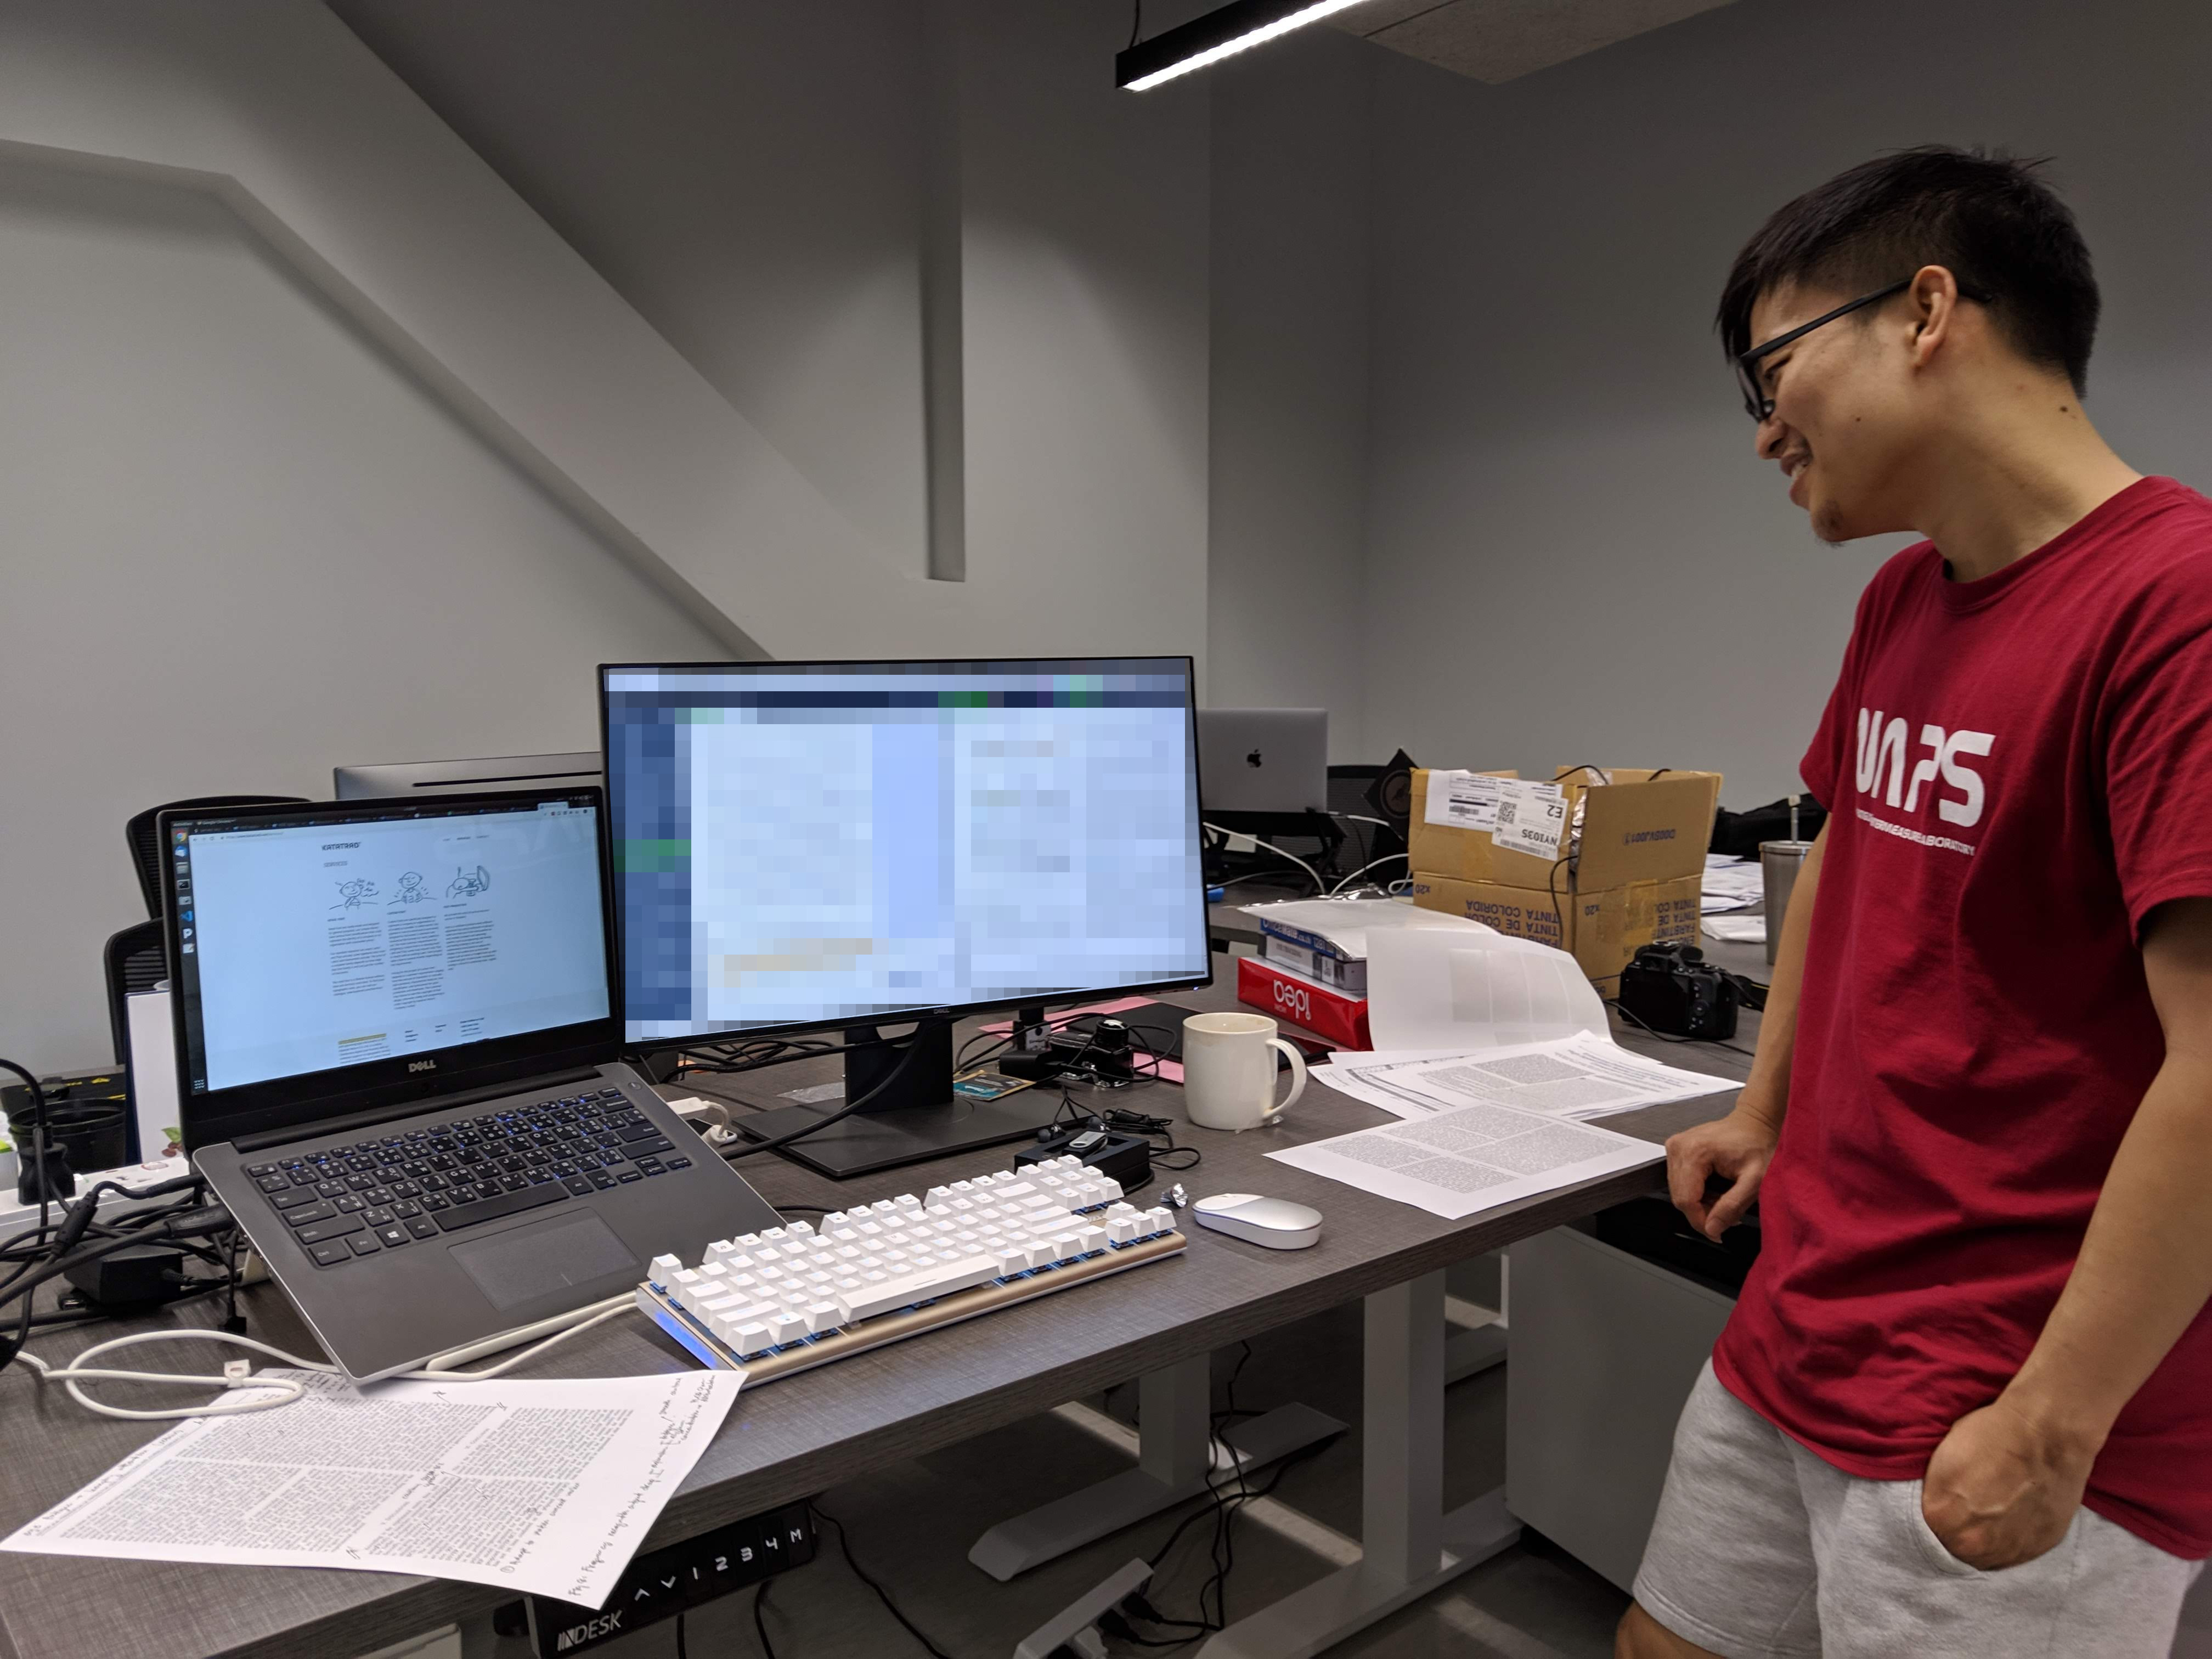
\includegraphics[width=0.55\textwidth]{/home/srakrn/Works/senior/internship/internship_report/diary/images/IMG_20190624_153749.jpg}
    \caption{อาจารย์ธีรวิทย์ วิไลประสิทธิ์พร ขณะทบทวนงานวิจัยโดยคร่าว}
\end{figure}

\section*{ภาพการฝึกงานวันที่ 8/7/2562}
\begin{figure}[H]
    \centering
    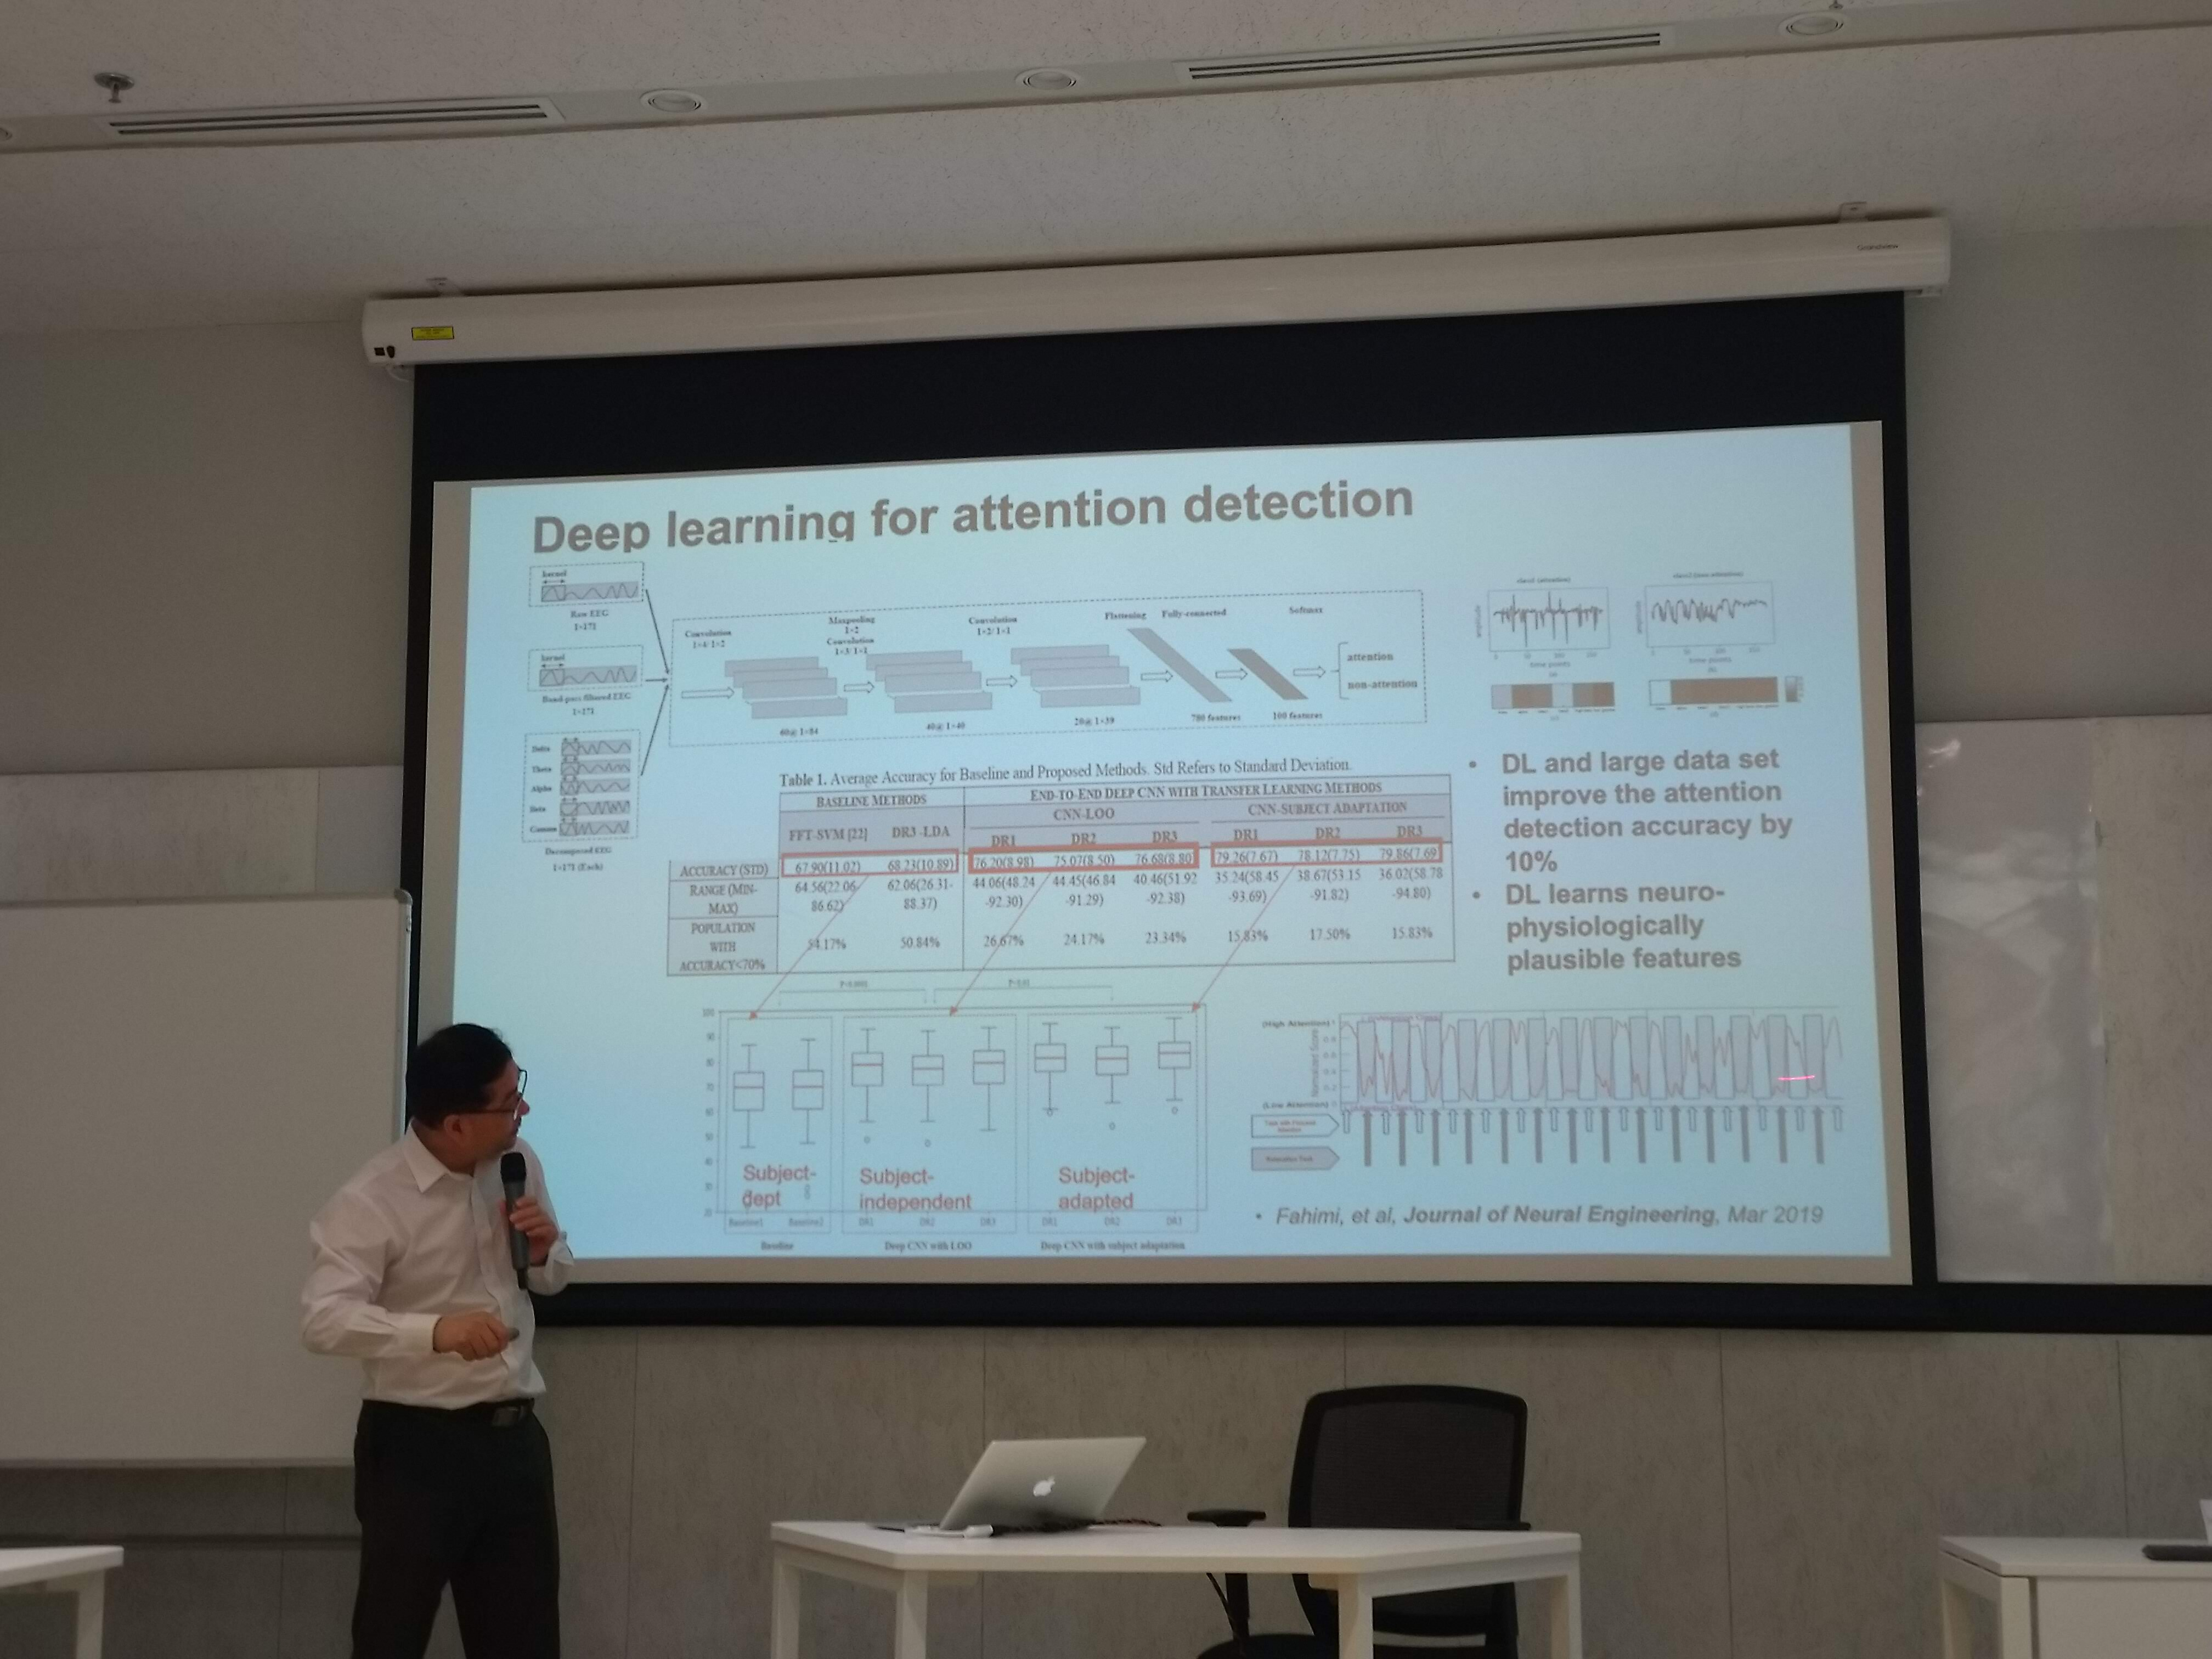
\includegraphics[width=0.55\textwidth]{/home/srakrn/Works/senior/internship/internship_report/diary/images/IMG_20190708_104544.jpg}
    \caption{บรรยายจาก Prof Guan Cuntai}
\end{figure}

\section*{ภาพการฝึกงานวันที่ 23/7/2562}
\begin{figure}[H]
    \centering
    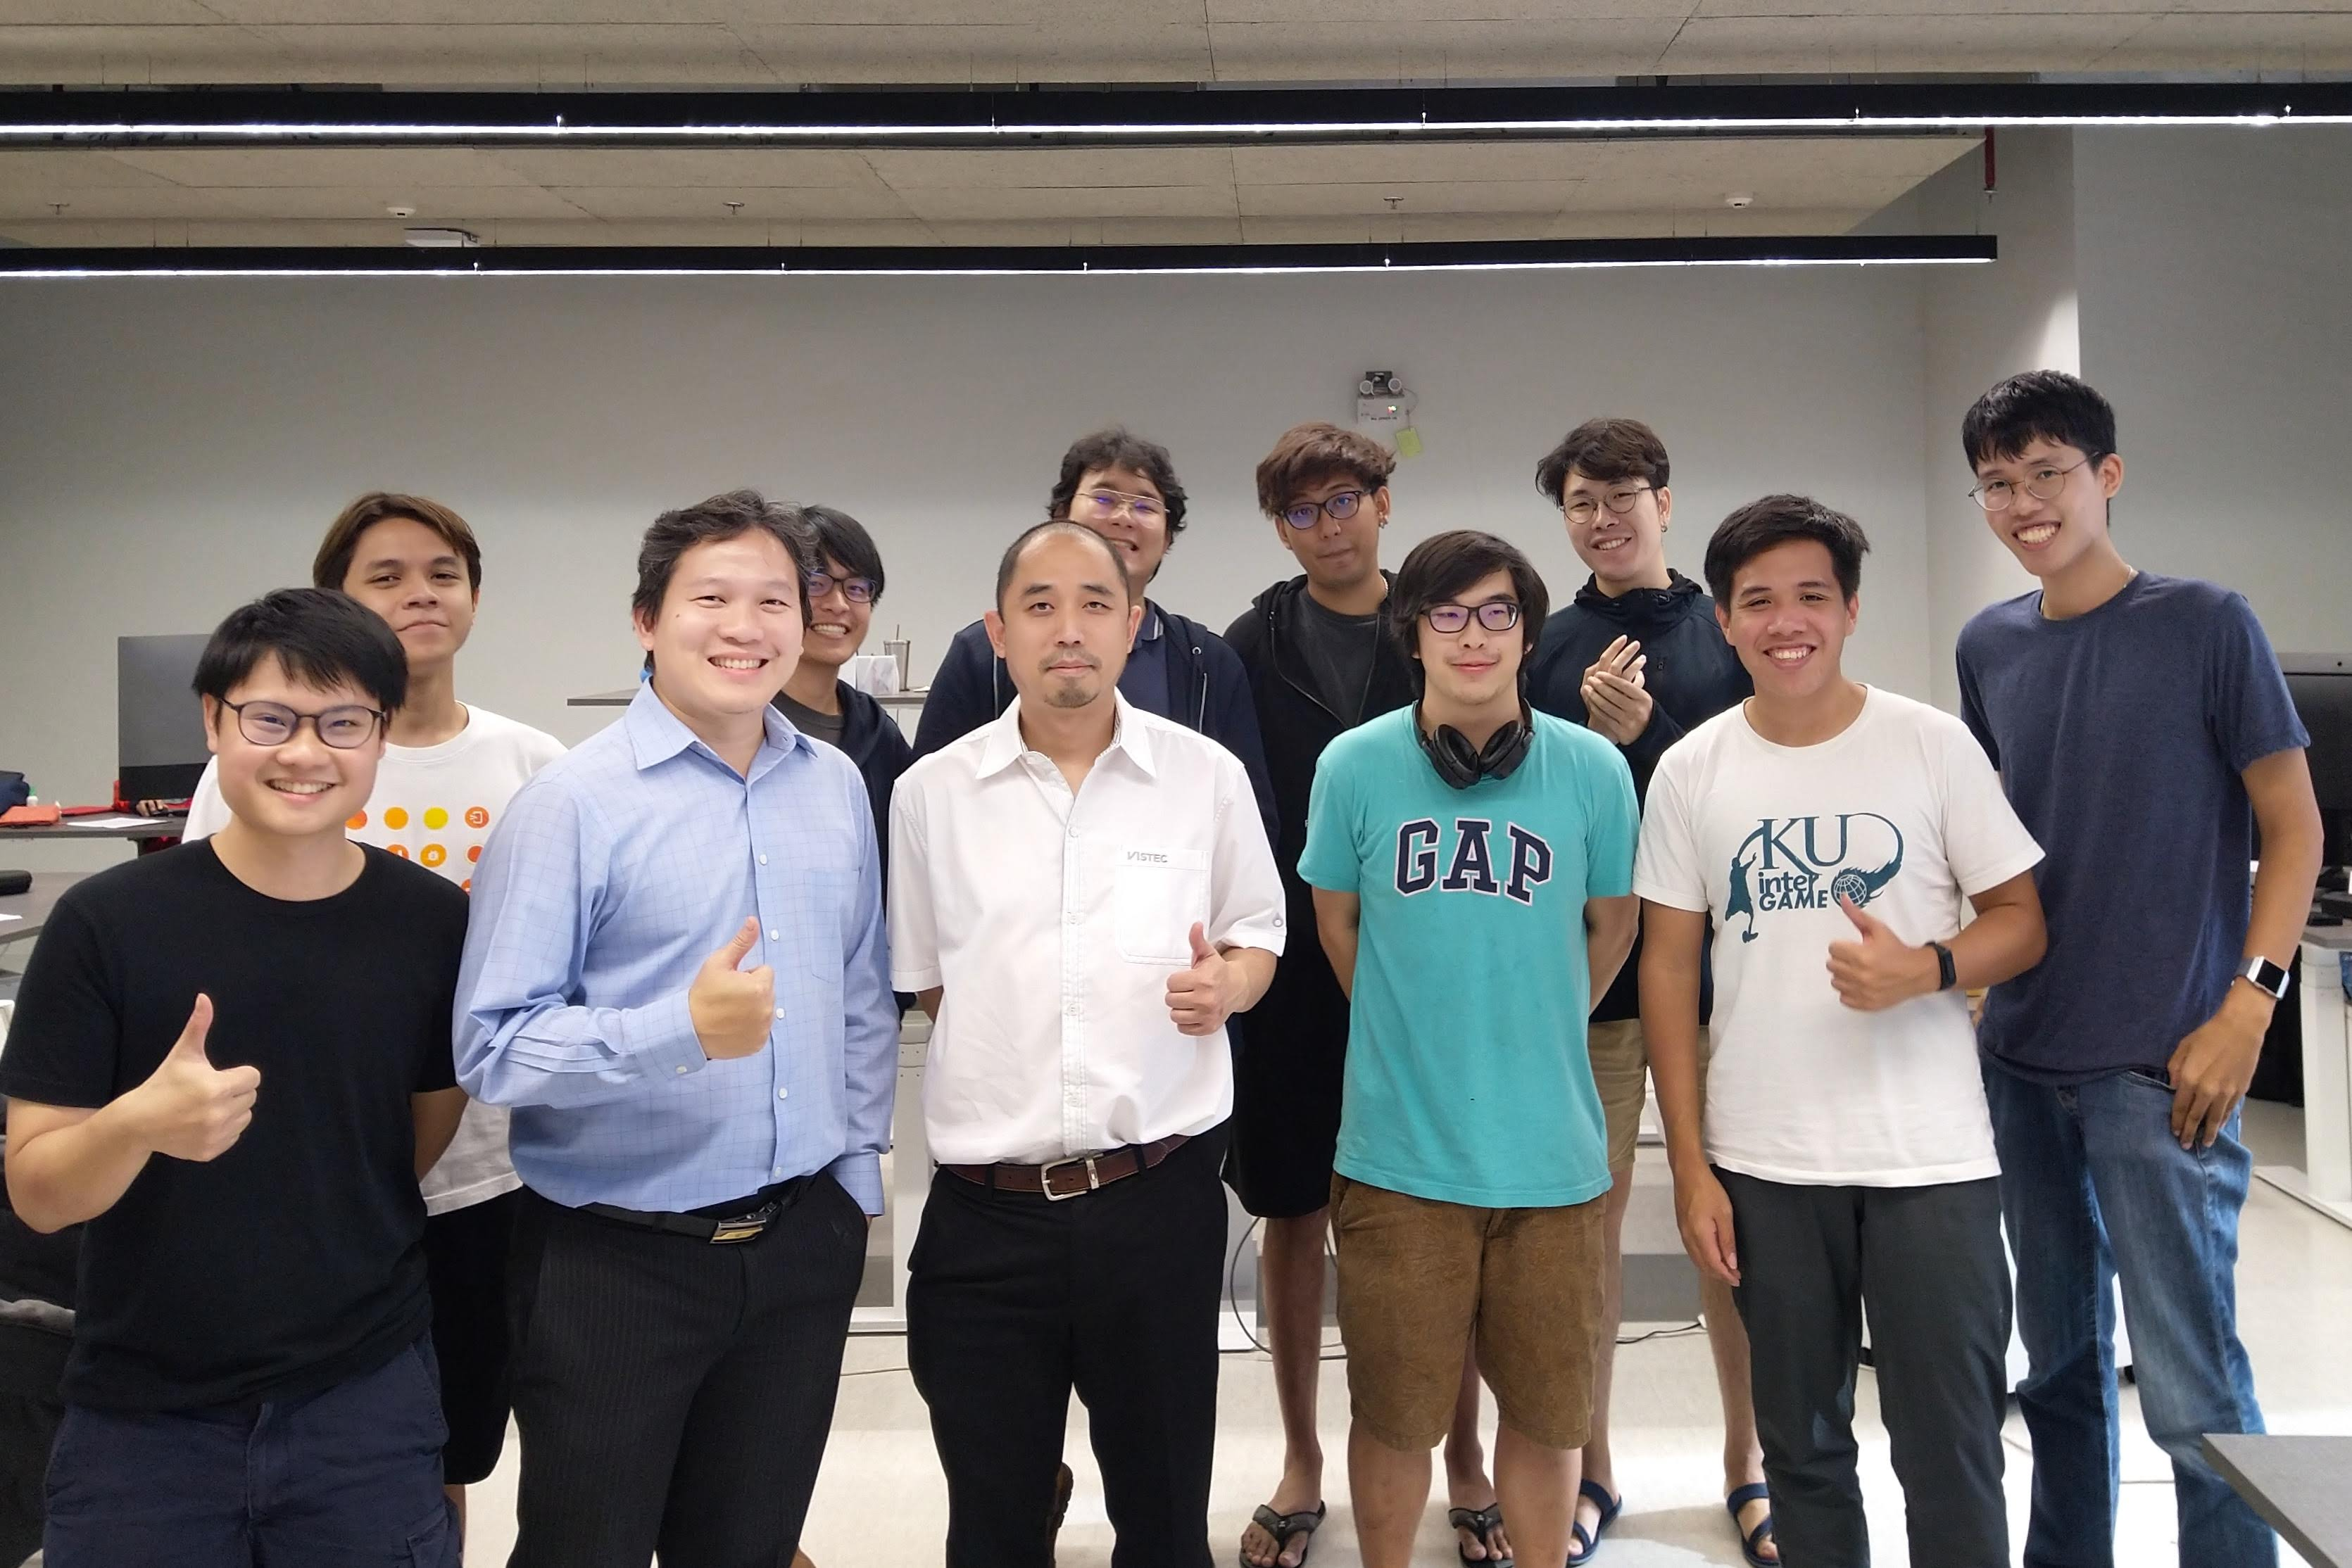
\includegraphics[width=0.55\textwidth]{/home/srakrn/Works/senior/internship/internship_report/diary/images/IMG_20190723_164246-01.jpeg}
    \caption{ทีมวิศวกรรมคอมพิวเตอร์เกษตรศาสตร์ ณ สถาบันวิทยสิริเมธี}
\end{figure}

\end{appendices}

\end{document}